%\documentclass{cumcmthesis}
\documentclass[withoutpreface,bwprint]{cumcmthesis} %去掉封面与编号页,电子版提交的时候使用。


\usepackage[framemethod=TikZ]{mdframed}
\usepackage{url}   % 网页链接
\usepackage{subcaption} % 子标题
\title{多波束测线问题的模型设计与优化}
\tihao{B}
\baominghao{202315009099}
\schoolname{山东大学(威海)}
\membera{李雨萌}
\memberb{谷雨桐}
\memberc{周佳一}
\supervisor{王效强}
\yearinput{2023}
\monthinput{09}
\dayinput{10}

\begin{document}

 \maketitle
\thispagestyle{empty}
 \begin{abstract}
本文在多波束测量系统探测海洋深度的实际应用中,采用了平面几何、初等解析几何方法建立了测量船在沿测线方向探测海底坡面时,任一点处的测量覆盖宽度、任意两个平行探测点重叠率的计算模型。并采用优化、规划算法建立了在海底为坡面、曲面时的优化多波束测量系统测线布设的模型,并对模型进行了检验、误差分析与评价。

针对问题一:问题一题设测线的法平面与海底坡面的交线是一条理想斜线,要求求解在该竖直平面上各条测线测深的覆盖宽度及相邻条带之间重叠率。本文建立了角平分线求对边平面几何模型,推导出测点测深覆盖宽度W与测点水深D、坡度$\alpha$、换能器开角$\theta$的数学关系,并依此计算相邻条带之间重叠率$\eta$。最后依据题干给出的具体参数值求解出9条测线在该竖直平面的测深情况。观察结果,可以看出当测线间距一定时水深较深处,测线其与前一条测线的重叠率较大,水深较浅处,测线其与前一条测线的重叠率较小。

针对问题二:问题二要求求解海底为斜坡的矩形海域上某探测点的测深覆盖宽度。本文建立空间解析几何模型,利用空间直角坐标系,推导出海底斜坡与水平面的夹角$\alpha$,测线方向与海底坡面法向量的水平投影夹角$\beta$与任意测点水深D和该测线法平面与海底坡面的交线的水平夹角$\gamma$的数学关系,之后,结合问题一建立平面几何模型求解该测点的测深覆盖宽度。最后依据题干给出的具体参数值求解具体测点的覆盖宽度。当测线夹角为90°和270°时,测线上各测点水深相等,求解结果显示各测点测深覆盖宽度也相等,该结果也侧面检验了模型的合理性。

针对问题三:在规则矩形海域内,本文需要在一定的约束条件下,例如限定适当的重叠率范围$\eta$和要求覆盖全区域S,设计测线布设方式使测线总长度最小化。此问题可归类为传统的优化和规划问题,其中的关键步骤在证明当总区域面积一定时,各探测点点测深覆盖宽度越大则测线总长度越小;证明当测线方向垂直于坡面法向量时,探测点测深覆盖宽度最大,并由此对测线测深覆盖宽度进行约束,求解最小化测线的总长度的问题。最终得到的设计方案为34条平行测线,其总长为68海里。

针对问题四:问题四给出了某海域的单波束先验测深数据,并给定重叠率、漏测海域面积等约束,求最小测线总长度的优化问题。本文依据等高线设计算法,结合问题三的结论,找到深度梯度变化最大的方向,并垂直该方向设计测线。本题中通过Kriging网格化方法进一步插值处理,采用递归的方式来进行测线布设优化,最终得到该海域的测线总长度。

\keywords{初等解析几何\quad  优化算法\quad    多波束测线\quad    测绘技术\quad 梯度下降法\quad 插值法}
\end{abstract}

\setcounter{page}{1}
\section{问题重述与分析}
多波束测线是目前广泛应用的水体深度测量技术,其精确性、便捷性、经济性的特点受到了广大海洋科学工作者的青睐。该测深系统工作原理为:测量船行驶过程中,向与航迹垂直的平面内发射多条超声波束,再由接收换能器采集海底返回的声波,通过间隔时间与声速,我们可以得到测量船与多条测线测量处之间的距离,再由距离分布计算出该测线下的海底深度数据。通过多次多位置测量海水深度,进而得到海底地形数据。

\subsection{问题一}
题设垂直于测线的竖直平面与海底坡面的交线是一条理想斜线,该斜线与水平面的夹角为$\alpha$,根据坡度$\alpha$、测量船测线方向、换能器开角$\theta$、海域中心处水深DA=70m、测线距间距d等参数,建立数学模型,求解在该竖直平面上,每条测线的海水深度D、覆盖宽度W以及与前一条测线重叠率$\eta$,最佳重叠率为10\%到20\%。

本文根据平面几何知识,首先建立角平分线求对边的平面几何模型,推导出了依据坡度、换能器开角、海域中心点水深求解各测线在该竖直平面上的测线的海水深度D、覆盖宽度W以及与前一条测线重叠率$\eta$的模型。

最后依据题干给出的具体参数值:换能器的开角为 120°、坡度为 1.5 °、海域中心点处的海水深度为 70 m,利用已建立的几何模型,对其他测线在该竖直平面的海水深度(m)、覆盖宽度(m)、与前一条测线的重叠率(\%)共三个指标值进行求解。

\subsection{问题二}
题设给定一个矩形海域,该矩形海域的海底斜坡与水平面的夹角为$\alpha$,测线方向与海底坡面的法向量的水平投影夹角为$\beta$,要求建立数学模型,根据已给出的多波束换能器的开角角度、海底斜坡坡度、海域中心点处的海水深度、测点距海域中心点距离、测线方向与海底坡面的法向量的水平投影夹角角度,求解该测点的测深覆盖宽度。

本文建立了空间解析几何模型,首先推导出依据海底斜坡与水平面的夹角$\alpha$,测线方向与海底坡面的法向量的水平投影夹角$\beta$求解任意测点水深D和该测线的法平面和海底坡面的交线与水平面形成的夹角$\gamma$的模型,之后,结合问题一建立的依据水深、多波束换能器的开角角度、交线坡度求解测点测深覆盖宽度的角平分线算对边的平几何模型求解该测点的测深覆盖宽度。

最后依据题干给出的具体参数值:多波束换能器的开角为 120°,坡度为 1.5°,海域中心点处的海水深度为 120 m,求解不同测点和该测点测线不同方向夹角情况下的覆盖宽度。
\subsection{问题三}
本题要求在给定的规则矩形海域内设计测线,在所述的合适的重叠率$\eta$、覆盖区域S等约束条件之下,使得总测线长度尽可能短。这个问题属于传统的优化和规划问题范畴,它需要我们首先计算测线在该海域内不同方向上的测量范围和投影,然后通过分析海域内测线投影范围之间的关系来确定如何使测线长度最短。具体来说,本文将详细论述测线设计的具体方式与过程,以最大程度地减少总测线长度,同时确保每个区域都得到了足够的覆盖。最后得到总测线长度的结果。
\subsection{问题四}

问题四给出了某海域单波束测量测深数据,要求依此数据设计出合理的该海域多波束测深的测线设计。要求设计的测线方案尽可能扫描整个待测海域、相邻条带之间的重叠率尽量控制在20\%以下且测线的总长度尽可能短。之后,依此测线方案计算测线的总长度、漏测海区面积占比、重叠率超过20\%部分的总长度三个指标。

本文依附件数据绘制出该海域海底地形图,其形状为"倾斜的非对称马鞍面",相较于问题三中的简单地形,这个地形显然更加复杂和具有挑战性。该复杂性表现在地形的总体坡度变化较大,且相邻区块之间的坡度变化较小。为了有效处理这个复杂地形,本文采用递归的方法,旨在寻找梯度变化最小的边界,然后使用分割法将地形划分为两个独立区域,并分别进行详细分析。在进行地形数据的投影过程中,本文选择了微元法作为处理离散数据的方法,这有助于更准确地表示地形特征。微元法的使用使得我们能够精确地计算覆盖面积、重叠率以及其他相关结果,这些结果将在后续的分析中起到关键作用。


\section{模型假设}
1. 由于该应用场景中测量区域较小,且地球为一不规则类球体,因此本文中抽象模型空间为标准空间直角坐标系,忽略表面的曲率。

2. 假定海水介质均匀,海水声速恒定,忽略海洋、天气等因素产生的白噪声,假设声波动力系统理想。且假定相关测量仪器无误差。

3. 假设海洋表面无潮汐、无波浪,不会影响船只的行驶与颠簸,保证测量船只不会摇晃或颠簸。

4. 本文未考虑声波发射与回传的延迟、校验。

\section{符号说明与单位制}
\begin{table}[!htbp]
    \caption{符号说明}\label{tab:001} \centering
    \begin{tabular}{ccccc}
        \toprule[1.5pt]
        符号 & 意义  & 单位\\
        \midrule[1pt]
        W & 条带覆盖宽度 & 米/m\\
		$\theta$ & 换能器开角 & 度/°\\
		D & 测线中心点处水深 & 米/m\\
		$\eta$ & 相邻条带面积重叠率 & - \\
		d & 相邻测线间距 & 米/m\\
		$\alpha$ & 坡度 & 度/° \\
		$\beta$ & 测线方向夹角 & 度/°\\
		$\sigma$ & 测量误差 & 米/m \\
		$\phi$ & 横摇、纵倾误差 & 米/m \\
		$v$ & 海水声速 & 米每秒 m/s\\
		$m$&测线间坡度上升高度&米/m\\
		$y$&海拔底侧上升距离&米/m\\
		$x$&海拔高侧上升距离&米/m\\
		$\Delta H$&测线间平均偏差&米/m\\
		$\sigma$&标准差估计值&-\\
		$\delta$&相对标准误差&-\\

        \bottomrule[1.5pt]
    \end{tabular}
\end{table}
该节表内符号在以下章节中的公式旁均有解释。

\begin{table}[!htbp]
    \caption{单位换算}\label{tab:001} \centering
    \begin{tabular}{ccccc}
        \toprule[1.5pt]
        单位换算 & 符号表示  & 适用范围\\
        \midrule[1pt]
        1 海里=1852 米 & $1nmi=1852m$ & 原数据横、纵坐标单位是海里,海水深度单位是米 \\
        \bottomrule[1.5pt]
    \end{tabular}
\end{table}

\section{模型建立与求解}
本文中主要使用了几何相关知识与运筹学规划问题的相关知识进行推导与建立模型。在计算覆盖重叠率与覆盖宽度中,我们采用三角函数进行求解,在规划路线中,我们采用传统优化算法进行设计测绘系统。最后所建立的模型基本解决了题目所述的问题。
\subsection{问题一}
本文根据平面几何知识,建立平面几何模型,得到坡度、测量船测线方向、换能器开角、海域中心处水深D、测线距间距d与每条测线的覆盖宽度W、与前一条测线重叠率n的几何关系式,利用该关系式得到本问题的平面几何模型。

之后依据题干给出的具体参数值:换能器的开角为 120°、坡度为 1.5 °、海域中心点处的海水深度为 70 m,利用已建立的平面几何模型,对距中心点处距离分别为±200m、±400m、±600m、±800m的其他测线在该竖直平面的海水深度(m)、覆盖宽度(m)、与前一条测线的重叠率\%共三个指标值进行求解。
\subsubsection{覆盖宽度W公式推导}
在坡面上,我们取多波束测深条带长度的水平投影作为其覆盖宽度。对于一条测线,我们以在该竖直平面上测线水深为界,将其测深条带覆盖宽度分为左、右两部分。
\begin{figure}[H]
    \centering
    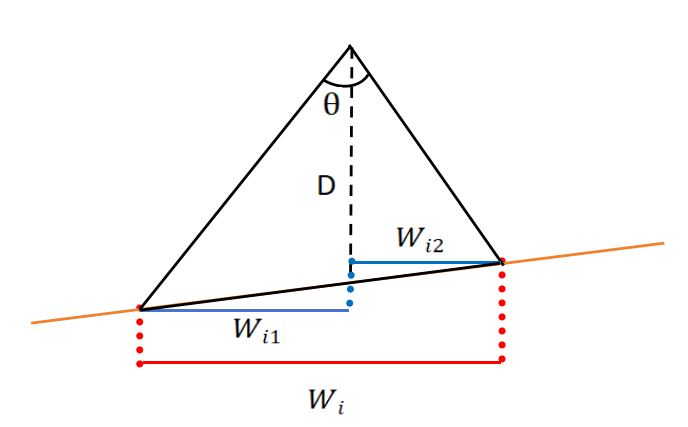
\includegraphics[width=.6\textwidth]{1}
    \caption{W宽度公式推导}
    \label{fig:one}
\end{figure}
\begin{equation}
W_{i}=W_{i1}+W_{i2}
\end{equation}
对于$W_{i1}$,我们可以得到:
\begin{equation}
tan\frac{\theta}{2}=\frac{W_{i1}}{D+x}, 0<\frac{\theta}{2}<\frac{\pi}{2}
\end{equation}
\begin{equation}
tan \alpha=\frac{x}{W_{i1}}, 0<\alpha<\frac{\pi}{2}
\end{equation}
联立上述两个公式,我们可以得到:
\begin{equation}
W_{i1}=\frac{D_itan\frac{\theta}{2}}{1-tan\alpha tan\frac{\theta}{2}}, subject\ to
\left\{
\begin{aligned}
tan\frac{\theta}{2}>0, \\
tan\alpha>0.
\end{aligned}
\right.
,
\end{equation}
\begin{figure}[!h]
    \centering
    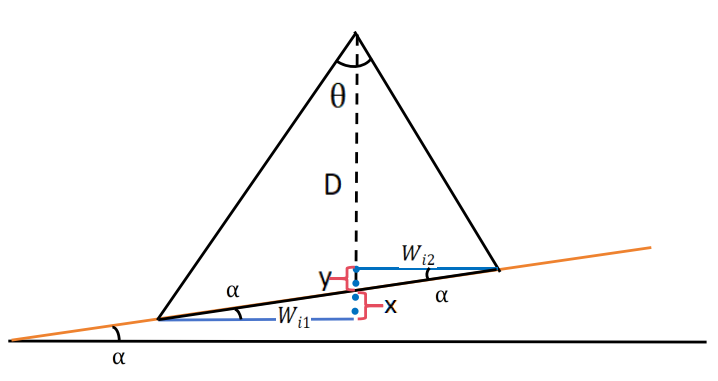
\includegraphics[width=.6\textwidth]{2}
    \caption{W宽度公式推导}
    \label{fig:two}
\end{figure}

同理,我们可以推导出$W_{i2}$的公式:
\begin{equation}
tan \alpha=\frac{x}{W_{i2}}, 0<\alpha<\frac{\pi}{2}
\end{equation}
\begin{equation}
tan\frac{\theta}{2}=\frac{W_{i2}}{D-y}, 0<\frac{\theta}{2}<\frac{\pi}{2}
\end{equation}
联立求解得到如下式子:
\begin{equation}
W_{i2}=\frac{D_itan\frac{\theta}{2}}{1+tan\frac{\theta}{2} tan\alpha}
\end{equation}

那么,根据$W_{i}=W_{i1}+W_{i2}$,我们可知:
\begin{equation}
\eta=\frac{W_{i2}+W_{(i+1)1}-d}{W_{i+1}}
\end{equation}
\subsubsection{相邻条带之间重叠率公式推导}
由题目已知条件可得:
\begin{equation}
l=W_{i2}-W_{(i+1)1}-d
\end{equation}
\begin{equation}
\eta=\frac{l}{W_{i+1}}
\end{equation}
\begin{figure}[H]
    \centering
    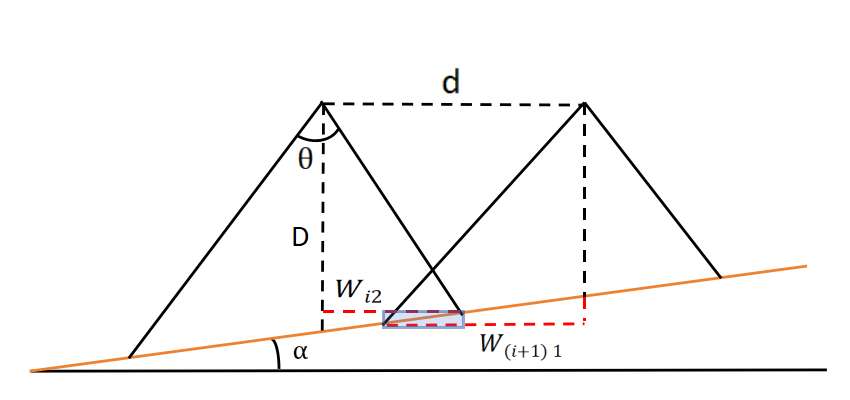
\includegraphics[width=.6\textwidth]{3}
    \caption{重叠率$\eta$公式推导}
    \label{fig:three}
\end{figure}

\subsubsection{各测线水深公式推导}
对于相邻测线,本文通过初等平面几何关系得到如下结论:
\begin{equation}
m=d\times tan\alpha
\end{equation}
\begin{equation}
D_{i+1}=D_i-m
\end{equation}
\begin{equation}
D_{i+1}=D_i-dtan\alpha
\end{equation}
\begin{figure}[H]
    \centering
    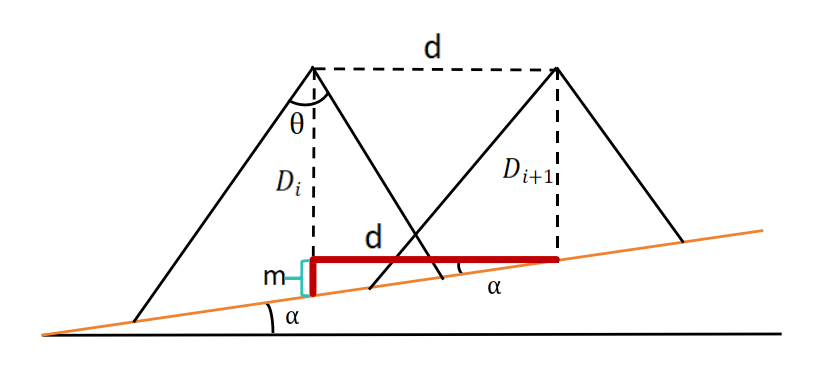
\includegraphics[width=.6\textwidth]{4}
    \caption{测线水深推导}
    \label{fig:four}
\end{figure}

对于非相邻测线,则易得:
\begin{equation}
d_n=nd(n\geq2)
\end{equation}
\begin{equation}
D_i=D-ndtan\alpha
\end{equation}
\subsubsection{问题求解}
由题设得:
\begin{equation}
\theta=120°\ \ \ \ \ \ \ \alpha=1.5
\end{equation}
\begin{equation}
D=70m\ \ \ \ \ \ \ \ d=200m
\end{equation}

将以上参数带入本小节所建立模型,对距中心点处距离分别为±200m、±400m、±600m、±800m的其他测线在该竖直平面的海水深度(m)、覆盖宽度(m)、与前一条测线的重叠率\%共三个指标值进行求解,结果见下表:
\begin{figure}[H]
    \centering
    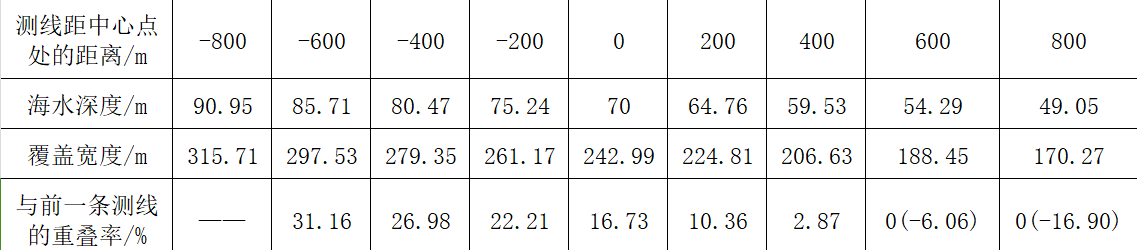
\includegraphics[width=.9\textwidth]{14}
    \caption{问题一求解结果}
    \label{fig:four}
\end{figure}
\subsubsection{结果分析}
规定由距中心点处距离为-800m指向800m为正方向,沿此方向海水深度由深至浅。

在距中心点处距离为-600m、-400m处的测线点位水深较深,其与前一条测线的重叠率较大,超出10\%—20\%的范围。

在距中心点处距离为-200m、0m、200m处的测线与前一条测线的重叠率位于10\%—20\%的范围之内。

在距中心点处距离为400m、600m、800m处的测线点位水深较浅,其与前一条测线的重叠率较低,低于10\%—20\%的范围,在距中心点处距离为600m、800m处测线与前一条测线的重叠率为负,出现漏测情况。

\subsection{问题二}
\subsubsection{模型建立}
题设给定一个矩形海域,该矩形海域的海底斜坡与水平面的夹角为$\alpha$,测线方向与海底坡面的法向量的水平投影夹角为$\beta$,本文建立了空间解析几何模型,利用该模型,可根据$\alpha$、$\beta$ 求解该矩形海域上任意一测点的水深D和与该测线的法平面和海底坡面的交线与水平面形成的夹角$\gamma$。利用水深D和夹角$\gamma$,依据问题一建立的角平分线求对边的平面几何模型求解该测点的测深覆盖宽度。

之后依据题干给出的具体参数值:多波束换能器的开角为 120°,坡度为 1.5°,海域中心点处的海水深度为 120 m,求解不同测点和该测点测线不同方向夹角情况下的覆盖宽度。
\subsubsection{该矩形海域内测点水深公式推导}
本文假设海面为一水平面,该矩形海域海底为与水平面夹角为的斜坡,该海域内各测点的水深不同。

给定的矩形海域海平面的中心点为A,过点A做垂直于海平面的竖直直线,交海底坡面于点O,线段$AO$长度即为A点水深$D_A$。过点O做平面$\pi$。平面$\pi$与海平面平行,平面$\pi$与海底坡面在水平面上的投影平行。

以点O为原点,海底坡面的法向量在平面上的投影为x轴,向量$\vec{OA}$为Z轴建立空间直角坐标系。
\begin{figure}[H]
    \centering
    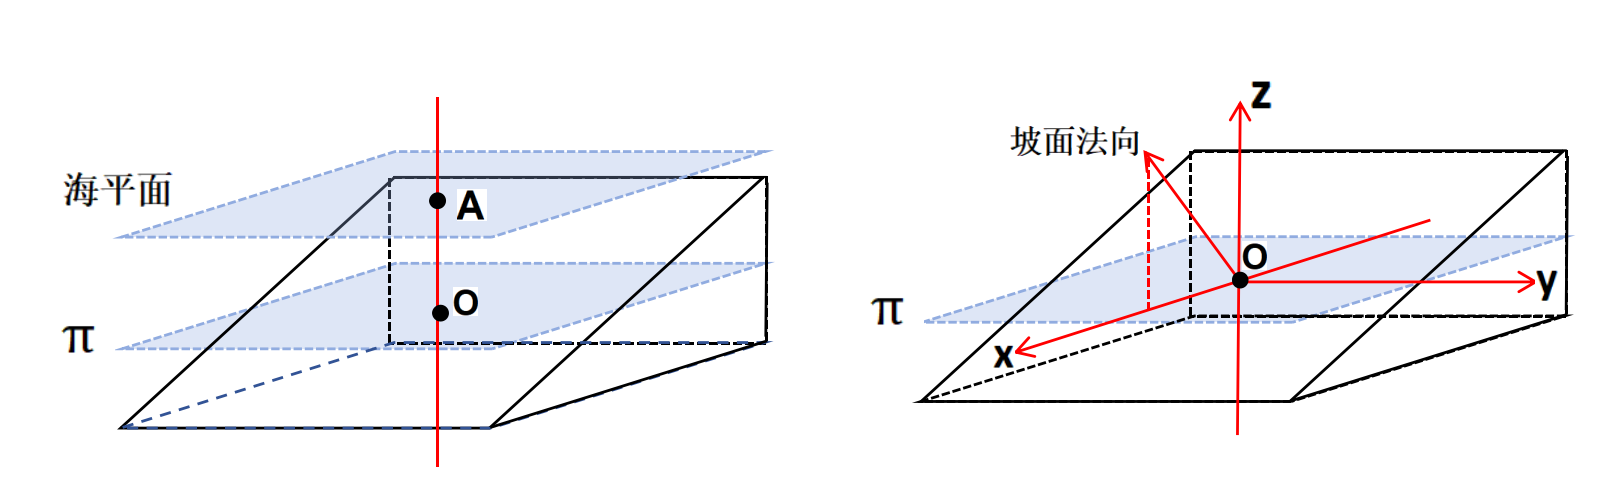
\includegraphics[width=.9\textwidth]{5}
    \caption{矩形海域测点水深推导}
    \label{fig:four}
\end{figure}

至此本文将海面上测量船航行情况映射至平面$\pi$。

由题意,测量船从海域中心A沿任意方向行驶距离d至B,向量$\vec{OB}$与x轴正方向形成的角度为$\beta$。

过点B做平面的垂线交于海底坡面于点C,其坐标为$(x_c,y_c,z_c)$,A、B处水深之差即为$-Z_C$。

过点B分别向x、y轴作垂线交轴于$x_0$、$y_0$,B点坐标为$(x_0,y_0)$。

由题意,海底坡面与水平面的夹角为$\alpha$。$By_0$与x轴平行,$\vec{BC}$与z轴平行,三角形$BCy_0$与海底坡面截面(两个绿色阴影三角形)平行且相似。由此可得:
\begin{equation}
tan\alpha=\frac{BC}{By_0}=\frac{-Z_c}{x_0}
\end{equation}
\begin{figure}[H]
    \centering
    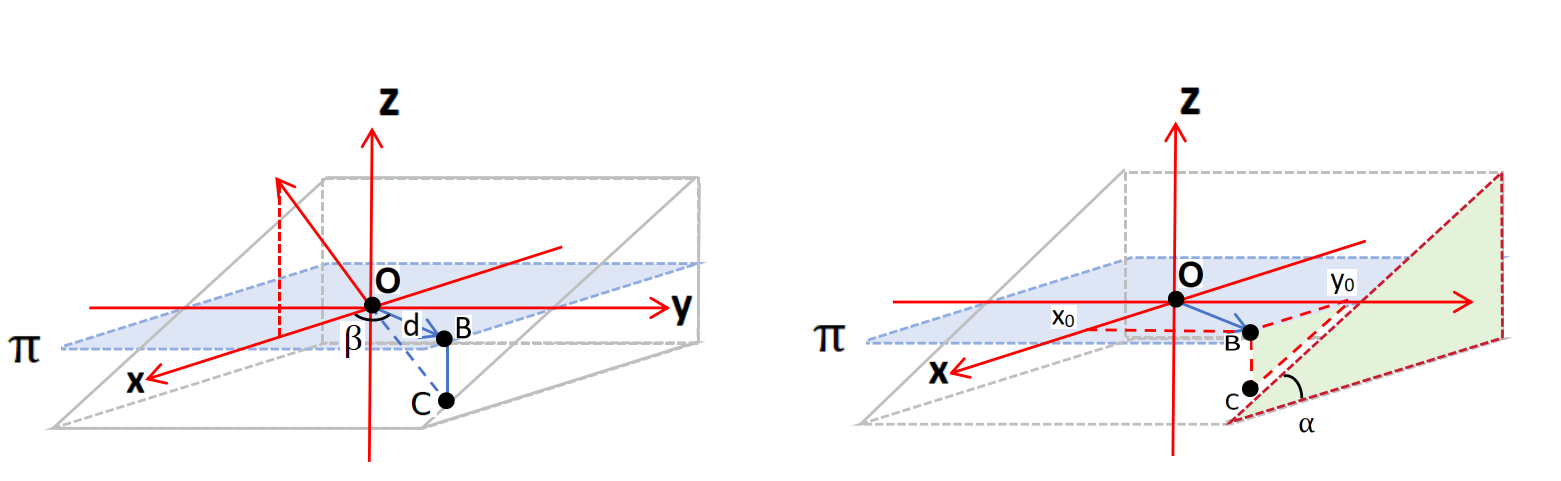
\includegraphics[width=.9\textwidth]{6}
    \caption{矩形海域测点水深推导}
    \label{fig:four}
\end{figure}

由题意向量$\vec{OB}$与x轴正方向形成的角度为$\beta$,由此可得:
\begin{equation}
cos\beta=\frac{Ox_0}{OB}=\frac{x_0}{d}
\end{equation}
\begin{figure}[H]
    \centering
    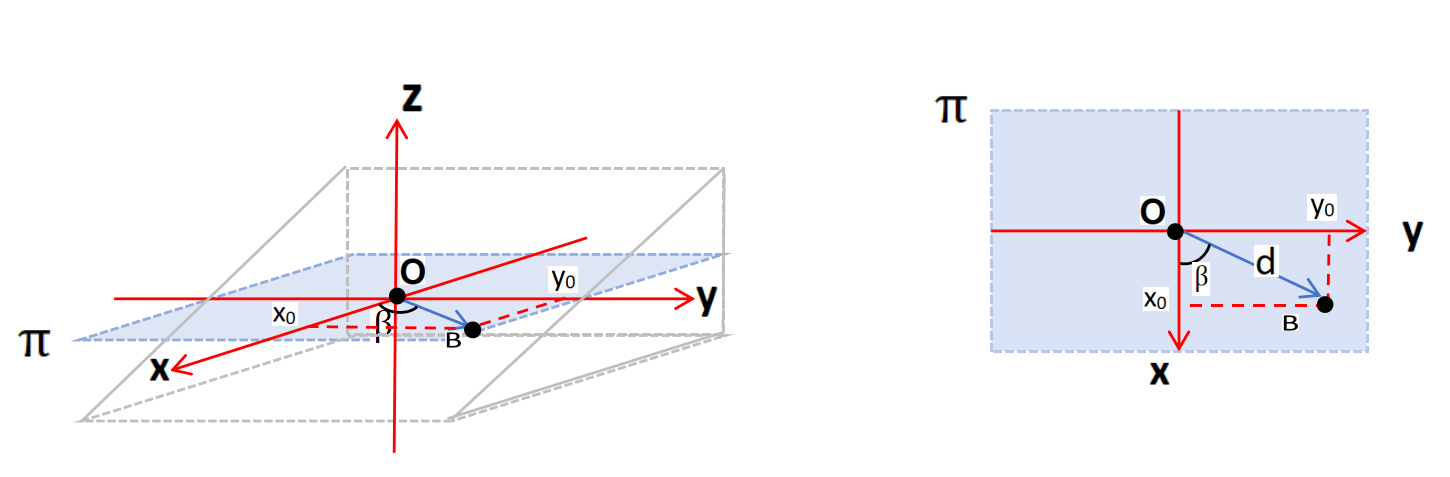
\includegraphics[width=.9\textwidth]{7}
    \caption{矩形海域测点水深推导}
    \label{fig:four}
\end{figure}

联立上述两式得:
\begin{equation}
-z_c=d tan\alpha cos\beta
\end{equation}
则B处水深为:
\begin{equation}
D_B=D_A+dtan\alpha cos\beta
\end{equation}
\subsubsection{该矩形海域内测点测深覆盖宽度推导}
在沿-z方向的俯视图上,过点O做OB的垂线OP,延长$Bx_0$交$\vec{OP}$于点P。$\vec{OP}$与y轴负方向形成的夹角大小与$\beta$相等,则$\angle OPB=\angle \beta$。由此可得:
\begin{equation}
tan\angle OPB=\frac{OB}{OP}=\frac{d}{OP}=tan\beta
\end{equation}
\begin{equation}
sin\angle OPB=\frac{x_0}{OP}=sin\beta
\end{equation}
\begin{figure}[H]
    \centering
    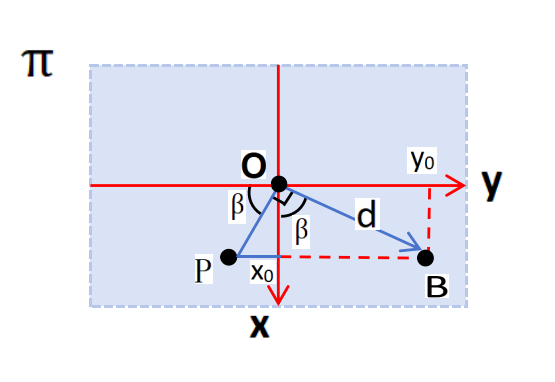
\includegraphics[width=.4\textwidth]{8}
    \caption{矩形海域测点覆盖宽度推导}
    \label{fig:four}
\end{figure}

过点P做平面$\pi$ 的垂线交海底坡面于Q,连接PQ。PB $\parallel$ x轴,则PQ=BC。
PQ$\perp$,则PQ$\perp$OB,又因为OP$\perp$OB,则OB$\perp$平面OPQ。面OPQ即为此测线的法平面。
OQ为测线法平面与海底坡面的交线,OQ与水平面的夹角$\gamma$ 即为问题一求解侧身覆盖宽度模型的坡度。
\begin{equation}
tan\gamma=\frac{PQ}{OP}=\frac{BC}{OP}
\end{equation}
\begin{figure}[H]
    \centering
    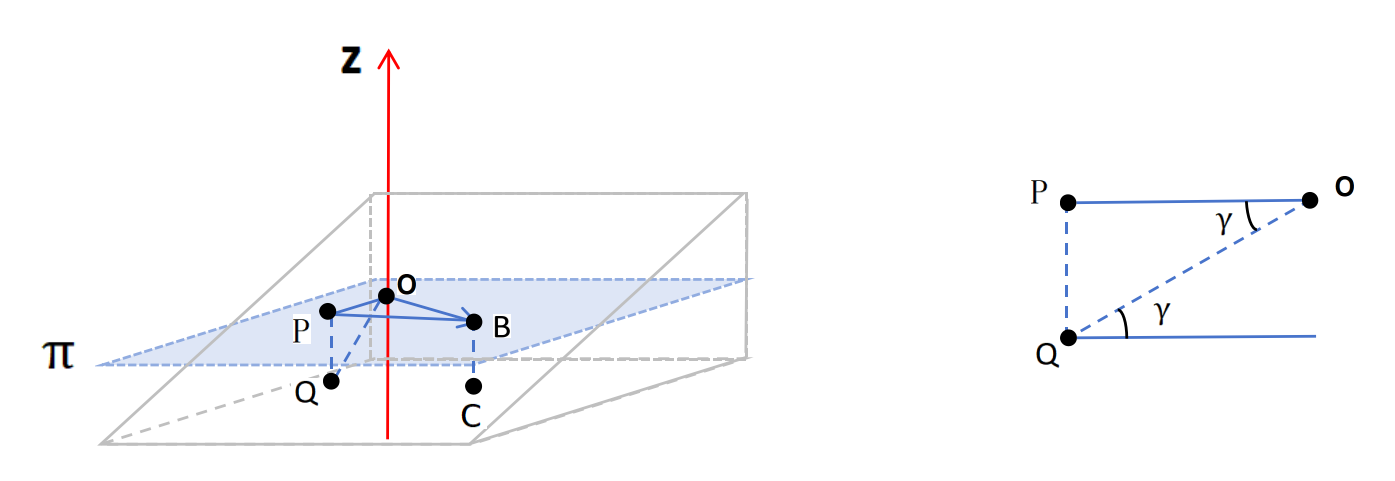
\includegraphics[width=.9\textwidth]{9}
    \caption{矩形海域测点覆盖宽度推导}
    \label{fig:four}
\end{figure}
联立上述四等式得到:
\begin{equation}
tan\gamma=tan\alpha tan\beta
\end{equation}
观察该式,发现$\gamma$的取值只与$\alpha $和$\beta$ 有关,则测量船在海面沿某一测线行驶时,与测线的法平面和海底坡面的交线始终是一条斜直线,且与水平面形成的夹角始终不变。因此,我们可以利用问题一建立的根据某测点的水深D以及与测线方向垂直的平面和海底坡面的交线和水平面的夹角求解该测点的多波束测深的覆盖宽度。
\begin{equation}
\left\{
\begin{aligned}
W_i=W_{i1}+W_{i2}=D_i\ tan\frac{\theta}{2}(\frac{1}{1-tan\gamma tan\frac{\theta}{2}}+\frac{1}{1+tan\gamma tan\frac{\theta}{2}})\\
tan\gamma=tan\alpha\ sin\beta\\
D_i=D_A+d\ tan\alpha cos\beta
\end{aligned}
\right.
,
\end{equation}
因此,可以推导得到:
\begin{equation}
W_i=(D_A+x\ tan\alpha)\times tan{\frac{\theta}{2}}\times \frac{2}{1-sin^2{\beta}tan^2{\alpha}tan^2{\frac{\theta}{2}}}
\end{equation}
\subsubsection{模型求解}
将题干中给出多波束换能器的开角为120°,坡度为 1.5°,海域中心点处的海水深度为 120 m,要求求解d=0、0.3、0.6、0.9、1.2、1.5、1.8、2.1海里和$\beta$=0、45、90、135、180、225、270、315°时的测深覆盖宽度,共64个结果。
将$\theta$=120°、$\alpha$= 1.5°、$D_A$=120m、d、$\beta$代入上式进行求解,结果见下表。
\begin{figure}[H]
    \centering
    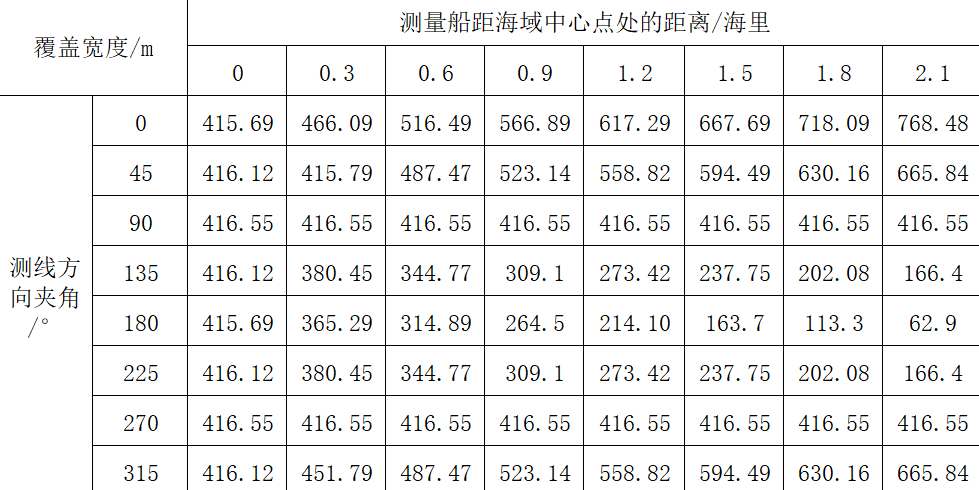
\includegraphics[width=.9\textwidth]{15}
    \caption{问题二求解结果}
    \label{fig:four}
\end{figure}
\subsubsection{结果分析}
观察求解表格,当测点距海域中心点处距离为0,即d=0时,测线夹角为90°和270°时,测点测深覆盖宽度最大。此时测线平行于矩形海域边界且测线上各测点的水深相等。

当测线夹角为90°和270°时,测线上各测点的测深覆盖宽度是相等的。

结合矩形海域内测点测深覆盖模型,当$\alpha $、$\beta$ 、$\theta$ 、$D_A$固定时测点的覆盖宽度只与该测点的水深有关。测线夹角为90°和270°时,测线上各测点的水深相等,各测点的测深覆盖宽度也相等,该结果也侧面检验了模型的合理性。

\subsection{问题三}
\subsubsection{模型建立与推导}
题设某矩形海域长 2 海里、宽 4 海里,海域海底西深东浅, 坡度为 1.5°。要求在此海域上设计测线进行多波束测线测量,在满足探测宽度覆盖全部海域,且相邻条带的重叠率保持在10\%到20\%以内的情况下,尽可能使测线总长度最短。分析问题可知,在相邻两测线重叠率理想的情况下,总探测宽度覆盖海域的面积M应该达到大约110\%到120\%的海域总面积,本文将此总探测宽度覆盖海域的面积M视为定值。M与测线长度L有如下关系:
\begin{equation}
\sum_{i=1}^{n}{\int_{L_i}{W}\,dx}=M
\end{equation}
由第二类曲线积分定理可得:该积分式满足全微分形式,可以化为如下二元积分变限函数的累计求和:
\begin{equation}
\sum_{i=1}^{n}{\int_{L_0}^{L_x}{W}\,dx}=M
\end{equation}
而M为一定值,对含参x的积分公式可以推导得出:当W的函数值增大时,$L_x$的值相应减小。因此,本章节可抽象该问题为:W为最大值时,$L_x$所要取到的值。本题要求所设计的测线测量长度最短,即:
\begin{equation}
\sum_{i=1}^{n}{|L_i|}
\end{equation}
值最小。
由数学分析知识得,当M一定时,W最大时,$\sum_{i=1}^{n}{|L_i|}$值最小。

给定的矩形海域海平面的中心点为A,过点A做垂直于海平面的竖直直线,交海底坡面于点O,线段AO长度即为A点水深$D_A$。过点O做平面$\pi$。平面$\pi$ 与海平面平行,平面$\pi$ 与海底坡面在水平面上的投影平行。

在平面上$\pi$,以点O为原点,沿东西方向做x轴,建立平面直角坐标系。为简化问题,本文将海面上测量船航行情况映射至平面,海面上任意一点可映射至平面,其坐标为(x,y)。
\begin{figure}[H]
    \centering
    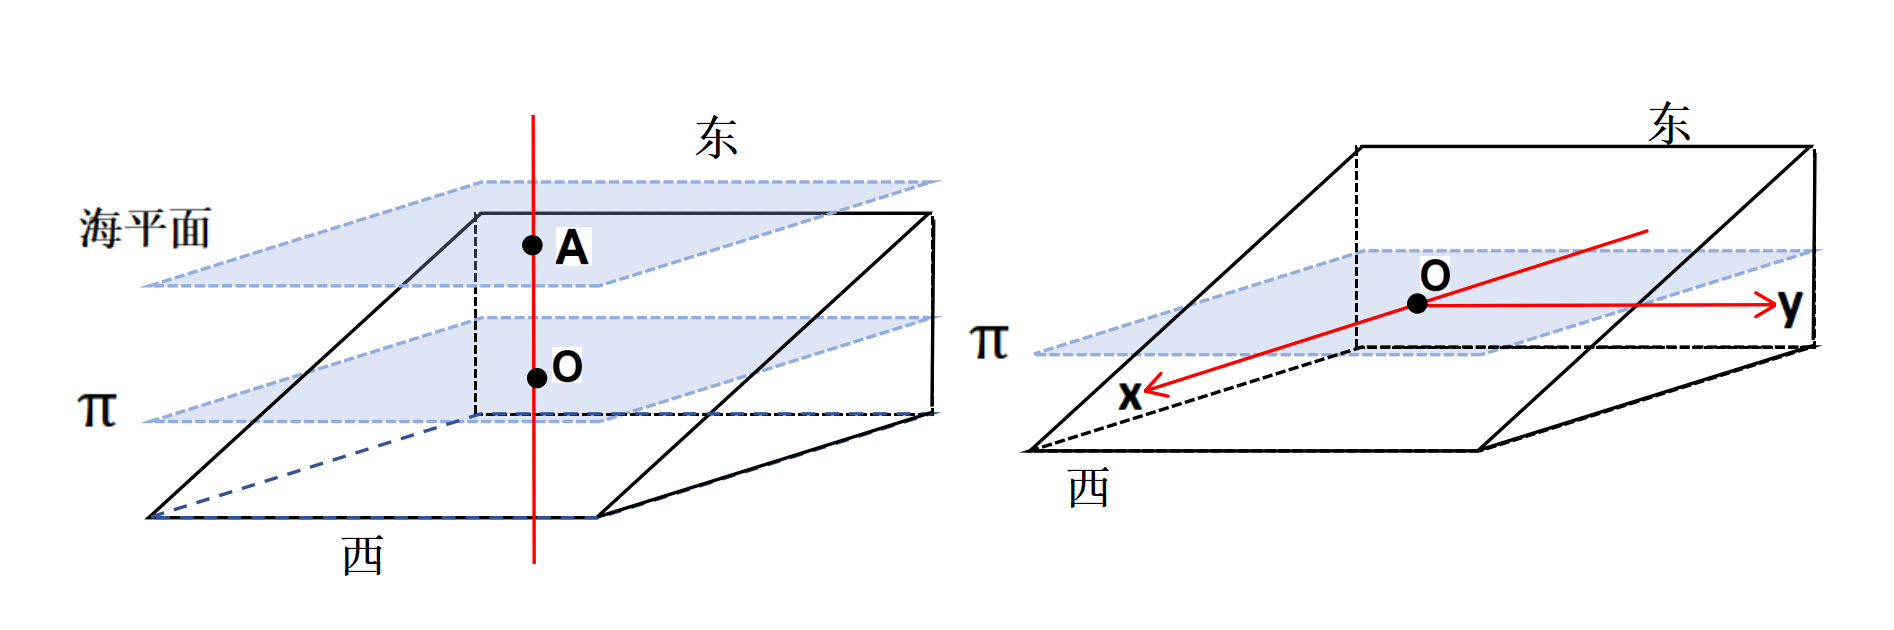
\includegraphics[width=.9\textwidth]{22}
    \caption{}
    \label{fig:four}
\end{figure}
根据第二问模型结果中海域中心点处的坡度与覆盖面积的关系,可以初步看出,当测线方向与坡面法线方向垂直的时候,同一个点处发射出的多波束探测的覆盖宽度最大,本问将给出数学证明。已知由前文推出的覆盖宽度关系式:
\begin{equation}
W_i=(D_A+x\ tan\alpha)\times tan{\frac{\theta}{2}}\times \frac{2}{1-sin^2{\beta}tan^2{\alpha}tan^2{\frac{\theta}{2}}}
\end{equation}
因为$D_A$=110m,$\alpha=1.5°$,$\theta=120°$三个参数本题题干均已给出给出,将三个参数代入,得W是关于横坐标x和测线方向与海底坡面的法向量的水平投影夹角为$\beta$的二元函数,记为W(x,$\beta$)。对于同一测点,$sin^2\beta$最大时W取得最大值。此时$\beta=90°$、$\beta=270°$。测线方向与y轴平行,与坡面法向垂直,沿南北方向。

\subsubsection{约束条件与优化模型}
由题设与上一小节的推导,可以抽象出如下约束条件,其中$x_i$为实数变量,表示题目所述问题中的实际值。
\begin{equation}
\left\{
\begin{aligned}
y_i(x_{i+1}-x_i)\geq0\\
y_i(-x_0+k_1\times x_o+b_1-2\times1852)\geq0\\
y_i(x_{n-1}+k_2\times x_{n-1}+b_2-2\times1852)\geq0\\
y_i({x_i+2\times1852})\geq0\\
y_i(-x_i+2\times1852)\geq0\\
y_i((k_2+1)x_i+(k_1-0.1k-1)x_{i+1}-0.1b+b1+b2)\geq0\\
y_i(-(k_2+1)x_i-(k_1-0.2k-1)x_{i+1}+0.2b-b1-b2)\geq0
\end{aligned}
\right.
,
\end{equation}
$y_i$为布尔值,如果与$y_i$相乘的式子满足约束条件,则$y_i$的值为1(True),否则为0(False)。
若要得到的测线最短,可设目标函数为:
\begin{equation}
Minimize\ \ \ \sum_{i=0}^{n-1}{y_i}
\end{equation}
该整数规划模型将最小化满足约束条件的$x_i$的数量并尽量使得$\sum_{i=0}^{n-1}{y_i}$的数值最小,进而得到最优的x、y数值。
\subsubsection{模型求解}
将已知条件带入之后可得结果,得到:33个条带完全位于区域内,34个条带可以全覆盖该区域面积。测线总长度为68海里。部分结果展示如下(全部代码请详见附录):
\begin{figure}[H]
    \centering
    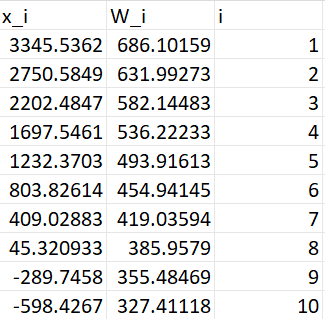
\includegraphics[width=.3\textwidth]{18}
    \caption{问题三求解结果部分展示}
    \label{fig:four}
\end{figure}
\subsubsection{结果分析}
通过结果表格和推导公式,我们得出了测得的海域面积为原本海域的109.47\%。这一结果表明了本文的测量方法较为准确和可靠。在假设平行与经纬线的条件下,得到的数据基本符合题目所述约束。
\subsection{问题四}

\subsubsection{地形坡度的建模方法}
\begin{figure}[H]
    \centering
    \begin{minipage}[c]{0.48\textwidth}
        \centering
        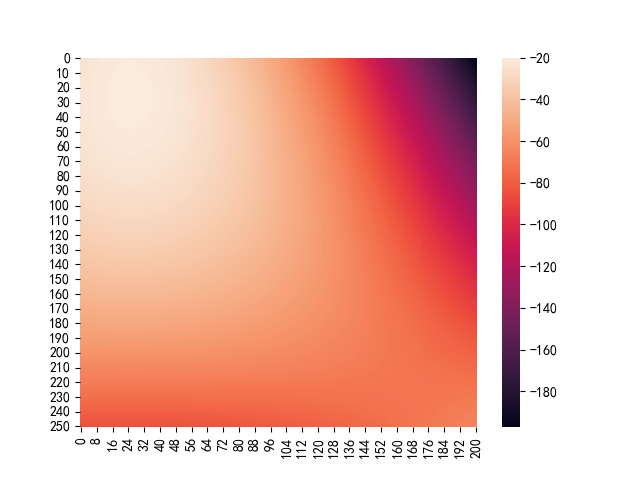
\includegraphics[height=0.18\textheight]{11}
        \subcaption{分层设色地形图}
    \end{minipage}
 \begin{minipage}[c]{0.48\textwidth}
        \centering
        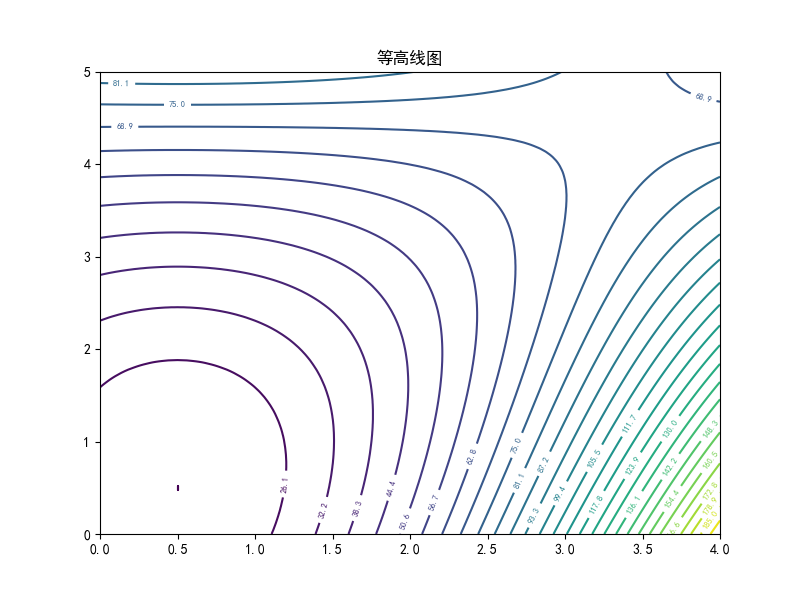
\includegraphics[height=0.18\textheight]{17}
        \subcaption{等深线地形图}
    \end{minipage}
    \begin{minipage}[c]{0.48\textwidth}
        \centering
        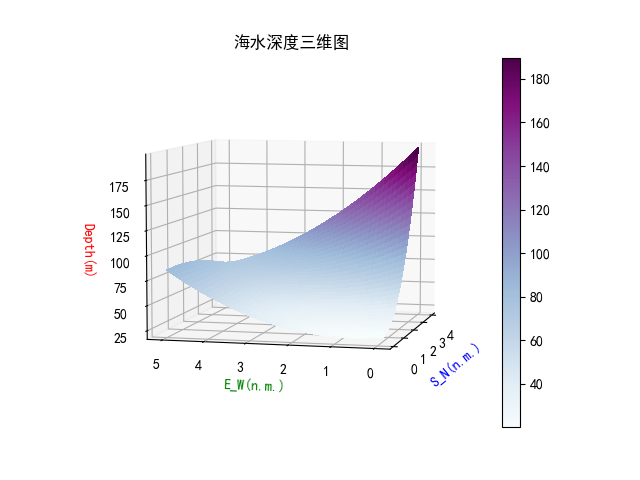
\includegraphics[height=0.18\textheight]{12}
        \subcaption{三维透视图1}
    \end{minipage}
\begin{minipage}[c]{0.48\textwidth}
        \centering
        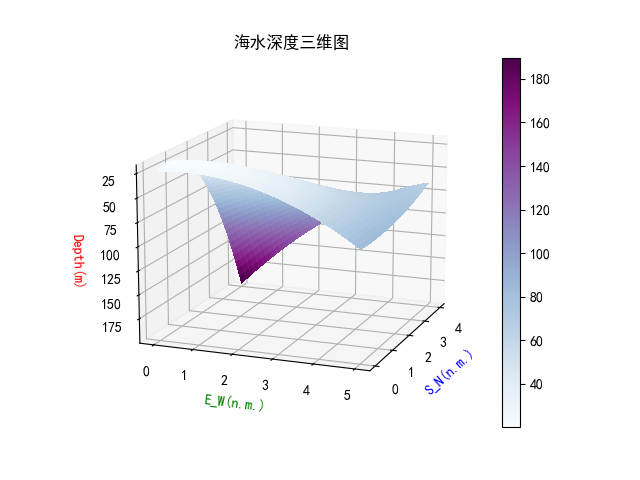
\includegraphics[height=0.18\textheight]{13}
        \subcaption{三维透视图2}
    \end{minipage}
    \caption{海底地形图像}
\end{figure}
在问题四给定的地形中,由于数据为离散化矩阵,非连续,且海底地形较为复杂,为不规则空间面。因此先对所给数据进行可视化,便于直观理解与分析,本文通过对数据的整体统计,得到了如下的等深线图与三维透视图:

分析图片可以大致观测海底曲面近似于不规则的马鞍形。所以在本小节的解答中,我们使用地形坡度$S$作为评判地形表面分析的重要依据,其中,$S$定义如下:[2]
\begin{equation}
S=\frac{360}{2\pi}arctan((\frac{\partial z}{\partial x})^2+(\frac{\partial z}{\partial y})^2)^{\frac{1}{2}}
\end{equation}
\begin{equation}
Slope_x = arctan(\sqrt{((\frac{\partial z}{\partial x})^2 + (\frac{\partial z}{\partial y})^2)})
\end{equation}
其中,$(\frac{\partial z}{\partial x})^2+(\frac{\partial z}{\partial y})^2$。

同样的步骤可以用于计算y方向的坡度分量。计算完x和y方向的坡度分量后,可以根据需要合并成总坡度或梯度。

由问题3的结论可知,当测线方向与海底最大坡度方向垂直时,单点的覆盖宽度最理想,线积分和最短,因此需要对海底坡面的梯度求最大值,认为当垂直于该梯度设计测线,可以达到较优的效果。

本题基于等高线图设计求解最大坡度的算法,由于给定数据为离散的空间网格上的点,难以直接使用微分计算梯度,因此设计新的算法求解最大坡度。易知当两个等高线间水平距离最短时,高度下降最快,此时梯度最大,可以将三维空间求梯度的问题降维简化为求平面上两曲线间最短距离的问题。因此设计算法求解等高线间最短距离,启发于支持向量机算法,对每个等高线上点在给定不同等高线标号作为标签的情况下,可以求解两类数据即两个等高线间最短距离。由于本题数据离散,等高线上不一定有合适的点能够求出最短等高线间距,因此还需要添加宽容度参数合理提取出能够反映等高线特征的点。

本题从两侧最低的角分别出发,求梯度最大的方向。以从全海域最低点$A_0(x_0,y_0,z_0)$出发为例,设定水深z每减小d米做一个等高线,则记目标为:
\begin{equation}
\left\{
\begin{aligned}
Z_0-id-c<Z_i<Z_0-id+c \\
min \sqrt{(x_i-x_{i-1})^2+(y-y_{i-1})^2}
\end{aligned}
\right.
,
\end{equation}
$A_i(x_i,y_i,z_i)$为第i条等高线容许范围内,与前一条等高线处选取的特征点水平距离最小的点。迭代求出所有$A_i$,并对其进行线性拟合,得到近似梯度最大的线,如图:
深水曲的梯度方向拟合直线表达式为:$y=-0.15\ x+0.69$
浅水区的梯度方向拟合直线表达式为:$y=-6.55\ x+4.53$
第j条测线为垂直于梯度拟合直线且交于点$B_j(x_j,y_j,z_j)$的直线,$y=x-(1+k)*x_j-b$

\begin{figure}[H]
    \centering
    \begin{minipage}[c]{0.48\textwidth}
        \centering
        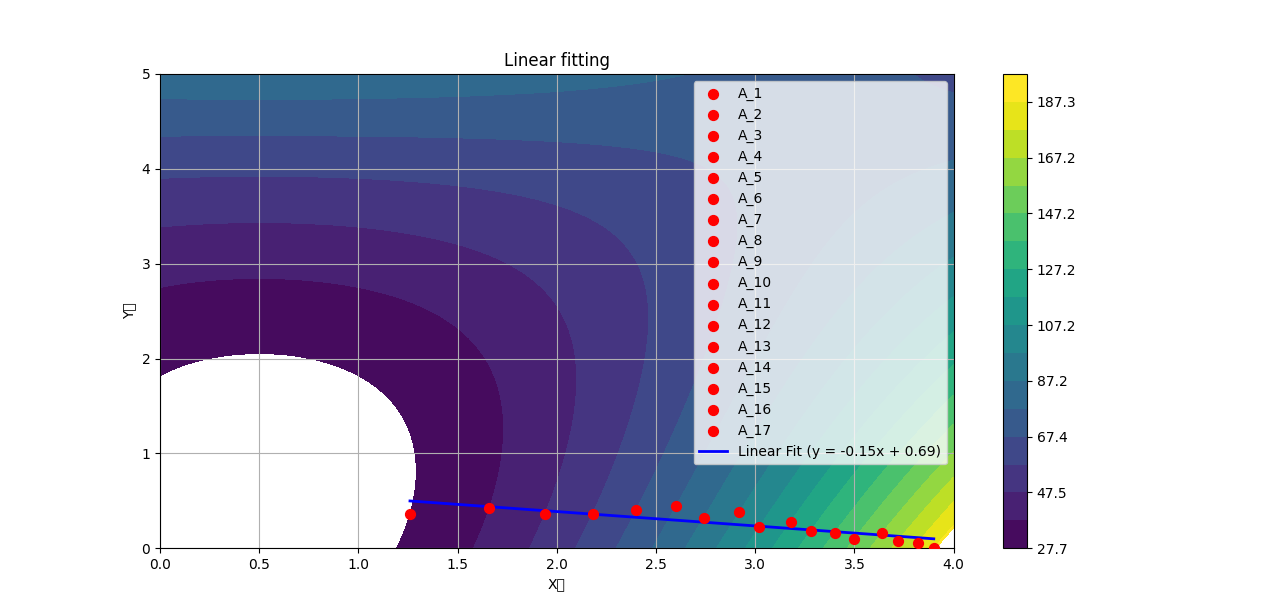
\includegraphics[height=0.20\textheight]{19}
        \subcaption{}
    \end{minipage}
 \begin{minipage}[c]{0.48\textwidth}
        \centering
        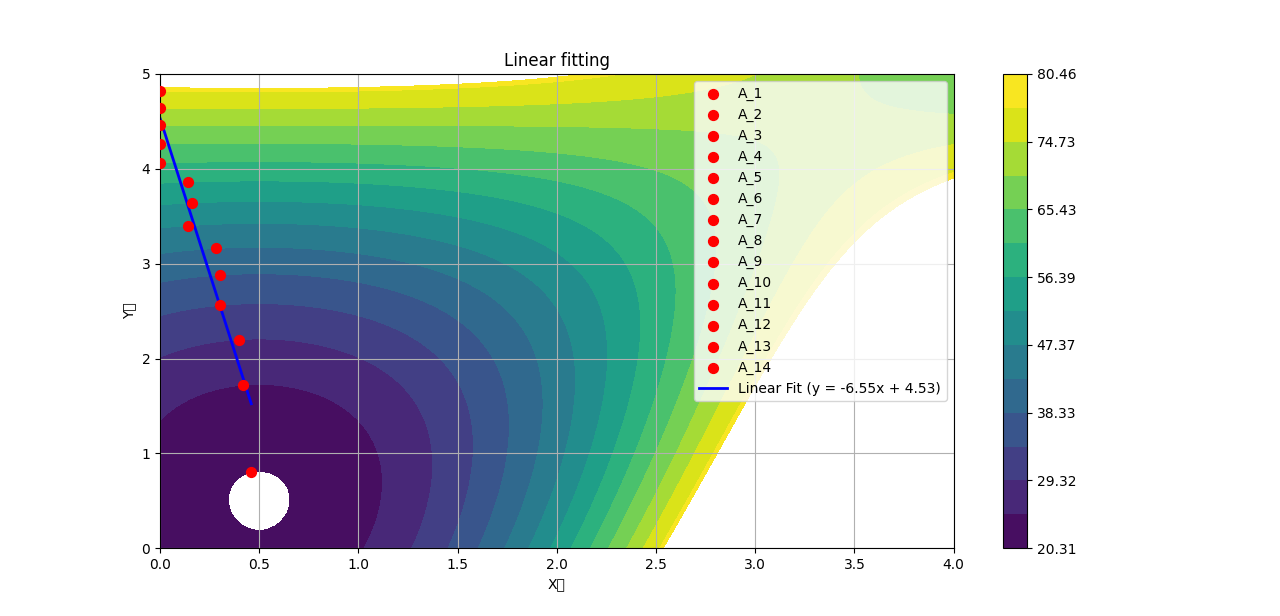
\includegraphics[height=0.20\textheight]{21}
        \subcaption{}
    \end{minipage}
    \caption{梯度下降最快方向的线性拟合}
\end{figure}
\subsubsection{Kriging网格化与测线的确立}
克里格(Kriging)法是目前广泛使用的网格化方法之一,具有较高的灵活性与准确性,其优势之一是可以在整体的测量与计算中基于较小的权重来补偿总体数据。由于在题设条件中深度数据的空间相关性较强,所以本文并不需要引入半变异函数。接下来,该方法需要根据半变异函数模型和数据点之间的距离,计算协方差矩阵。这个矩阵用于量化不同点之间的相关性,并在Kriging中进行权重分配。由于Kriging在插值运算的过程中,散布矩阵(协方差矩阵)对最终结果影响较大,则我们引入了Kriging插值方程组,$i=1,2,...,n$:
\begin{equation}
\left\{
\begin{aligned}
\sum_{j=1}^{n}{\lambda_j\gamma(x_i,x_j)+\mu=\gamma(x_i,x)}\\
\sum_{i=1}^{n}{\lambda_i}=1\\
\end{aligned}
\right.
,
\end{equation}
在插值的过程中,我们需要使用Kriging方法估计未知点的深度。Kriging考虑了数据点之间的空间相关性,并为每个未知点分配一个权重,根据其在空间上与已知点的距离和相关性来进行深度估计。这样,可以生成一个连续的海底深度表面模型。其中,插值条件为:
\begin{equation}
\gamma(h)=\frac{1}{2N(h)}\sum_{i=1}^{N(h)}{[z(x_i)-z(x_i+h)]^2}
\end{equation}


通过海底的深度矩阵数据,我们可以在梯度方向拟合直线上获得更多具有深度的三维空间上的点,因此可以对坡面梯度进行微分处理得到所需的坡度值$\alpha$ 。
可以定义自变量为(z,$\alpha$)的覆盖深度$W1_j,W2_j,W_j$

\subsubsection{模型求解}
因为本算法选取测线均垂直于基于等高线图求解的梯度最大方向拟合直线,所以认为测线几乎沿等深线前进,即深度z一定。又已经将类马鞍面的海底曲面沿山脊分成两个近似坡面,则认为沿侧线方向探测的法平面与海底截得坡面角度即为$\alpha$。则将测线探测的覆盖宽度转化为沿测线在测线与拟合直线交点处的探测宽度,将两测线的重叠率转化为拟合直线上两个点覆盖宽度的重合率,将测线探测的覆盖区域近似为长方形区域。从最低点开始,找到覆盖域刚好覆盖该边界点的测线,并将下一测线与该测线的重叠率限定在百分之13到17之间,求与该测线距离最远的满足重叠率要求的测线,并迭代求出区域内全部测线。
全海域内的测线分布图示如下:

\begin{figure}[H]
    \centering
    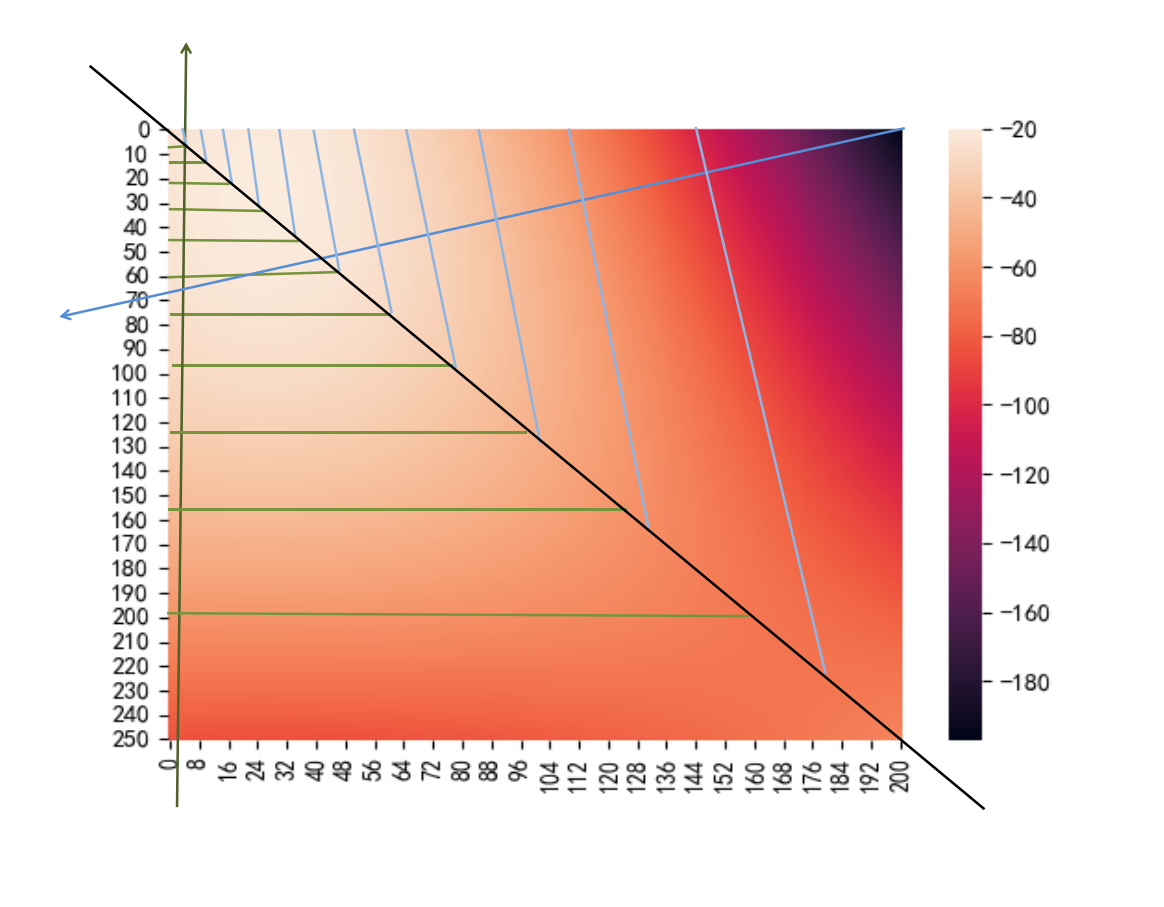
\includegraphics[width=.7\textwidth]{20}
    \caption{问题四测线示意图}
    \label{fig:four}
\end{figure}


\subsubsection{结果分析}
通过分析结果表格和推导公式,我们可以得出测得的结果为:测线的总长度为196.34海里,漏测海区占总待测海域面积的百分比为3.958\%,在重叠区域中,重叠率超过 20\%部分的总长度为8.38海里。这一结果表明,我们的测量方法在满足假设条件(即平行于经纬线)的情况下,表现出了相当高的准确性和可靠性,与问题陈述中的约束条件相符合。

这个测量结果反映了我们的方法对于复杂地理环境的适用性,并且与预期值相当接近,这进一步证明了本文中采用的测量方法的有效性。在考虑到海域的地理特征以及问题中的限制条件时,测量结果的准确性和一致性得到了验证,而本文方法得到了不错的结果。

a) 漏测面积计算评价模型

在多波束测量中,相邻波束的覆盖区域之间存在一定的重叠和缝隙现象。该重叠和缝隙问题是海底测量中的一个挑战,因为它可能导致某些海底区域未被测量,从而降低了海底地形测量的准确性和可靠性。在这一背景下,我们迫切需要采用漏测面积计算评价模型,以在一定的约束条件下,最大限度地减少漏测对测线覆盖范围的不利影响。在本文中问题三的解答中,通过进行漏测面积的约束,达到了测量完全海域面积的作用,并计算出来了最短的总测线长度l=68海里的结果。这个漏测问题的解决方案涉及到优化算法的应用,旨在通过运筹学和计算方法,在已知的约束条件下,尽量减小漏测面积。该漏测问题采用了优化算法,通过运筹计算尽可能在已有条件之下得到尽可能小的漏测面积。优化算法的引入使得漏测面积的评估有了理论依据与可用性检验。

b) 重叠率超20\%的长度评价模型

当重叠率较大时,能够使得多波束测绘计算的精度更高,而此时总测线长度也随之延长。本题的重叠率按照$\eta=\frac{W_{i2}+W_{(i+1)1}-d}{W_{i+1}}$定义,能够较好地得到相邻测线之间的测量区域的重叠率。当重叠率超过20\%时,数据存在较大的冗余,同时对较浅海域的测量有着提高精度的作用。然而,正如我们在问题四的解答中所观察到的,即使在重叠率较高的情况下,仍可能出现漏测面积相对较大的情况。这表明管理约束条件和精心规划测线路径对于多波束测绘至关重要。在实际操作中,需要综合考虑多个因素,如地形复杂性、资源可用性和预期精度,以确定最佳的测量策略。因此,对约束条件的管理与测线路线的规划就有着较高的设计要求,例如测线路线的规划需要考虑到地形特征、预期的重叠率、预先设计的测线路线等。本文问题四的解答中,计算得到的长度8.38海里。本模型引入了优化算法,在合适的条件下,通过计算重叠率超过20\%的总测线长度对测量较浅海域有着重要的作用。
\begin{figure}[H]
    \centering
    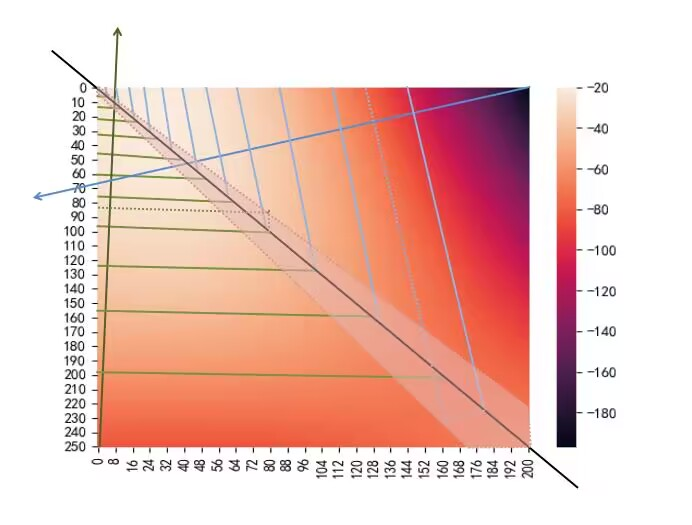
\includegraphics[width=.6\textwidth]{23}
    \caption{重叠区域示意图}
    \label{fig:four}
\end{figure}
\section{模型的分析与检验}
\subsection{模型的可行性检验}
在该多波束测深算法系统中,首先要证明该模型的正确性。可见,上文所述的数学推导,为该测量模型提供了理论基础,具有较强的数学理论依据。因此,本文模型正确,有着较强的可行性。
\subsection{模型可靠性检验}
下面介绍算法精度的评估方法。精度评估本质上是算法系统稳定性与可靠性的试验,其结果不仅能反映实际过程中测量时的误差(比如波浪导致的船体颠簸),也能验证算法本身的鲁棒健壮性。
\subsubsection{相对精度评估方法}
在多波束测量海底的过程中,边缘波束相对中央波束的声波返回时间将更长,这其中将会导致边缘波束测距值低于中央波束测距值,因此,我们需要进行中央波束与两侧波束测量的水深偏差进行合理评估与对比统计。
根据测线规划原则,测量时将采用部分重叠来进行规划相对精度的评估方法——也就是说:让相邻测线的两侧边缘波束与中央波束尽可能重合或平行,再规划平行于主测线的两侧边缘的校验用的测线。由于题目中规定,一般重叠率为10\%到20\%,重叠的测量覆盖区域则可用于误差的校验于估计。误差估计公式采用了改进的Bessel公式,对方差进行估计,其定义如下:

\begin{equation}
\Delta H=\frac{\sum_{i=1}{n}{m_i-n_i}}{k}=E[m_i-n_i]
\end{equation}
设$m_i, n_i,(i=1, 2, 3...k)$分别代表两主测线各自的水深,并取其中的k个测点,并且,$\Delta H_{mn}$和$\sigma_{mn}$分别表示两测线测量到的深度的平均偏差与标准差估计。
\begin{equation}
\sigma_{mn}=\sqrt{\frac{\sum_{i=1}{k}{\Delta H^2}}{2k}}=\sqrt{\frac{\sum_{i=1}{k}{(m_i-n_i)^2}}{2k}}
\end{equation}
之后进行标准化,使得计算结果落在$[0,1]$范围内,其中$\theta$为相对误差:
\begin{equation}
\delta=\frac{\sigma}{H}\times 100\%
\end{equation}
经过计算可知,本文所述模型的$\delta_{mn}$的值小于0.1,从方差估计来看,本文模型设计合理,具有较高的健壮性。[1]
\subsubsection{绝对精度评估方法}
仅对单个波束覆盖范围进行分析,选取相同波束测点进行评估,本文将使用IHO-44标准,计算最大误差与最小误差的限差:
\begin{equation}
H_{max}=max\{h_1,h_2,h_3...\}
\end{equation}
\begin{equation}
H_{min}=min\{h_1,h_2,h_3...\}
\end{equation}
上面定义了同波束测点水深数据的两个最值,下面计算限差:
\begin{equation}
\sigma_{max}=\sqrt{a^2+(b\times H_{max})^2}
\end{equation}
\begin{equation}
\sigma_{min}=\sqrt{a^2+(b\times H_{min})^2}
\end{equation}
由IHO-44标准与标准差估计可以得到如下约束条件:
\begin{equation}
\sigma_{min}<\sigma<\sigma_{max}
\end{equation}
根据计算,本文中的计算模型满足大于99.74\%置信度的标准差区间[3],因此,本文所述测量算法的精度基本满足现实研究。
\section{模型评价}

\subsection{模型优点}
1. 本文基于初等解析几何与传统优化算法,模型经典、可靠,具有较强的理论依据。在该实际应用问题中,我们通过该算法得到的数值解符合实际情况,能够合理地描述与计算出地理数据。因此,该算法基本符合上述实际问题的使用场景。

2. 本文在前三个问题中采用了连续化处理,使模型精度大大提高,并且可以通过分析手段来处理数据。而第四问的基于离散化数据,本文采用基本优化算法,,将大块面积切割成较小区域,迭代出最终结果,充分发挥了数据特征的优势,有效降低了数值计算的难度。

\subsection{模型缺点与改进}
1. 在实际生产研究中,难免遇到“非理想”情况,当测量区域较大时,我们需要考虑地面的弯曲,将投影面引入曲率的模型,需要根据场景建立三维极坐标。

2. 在本文设计模型中,可能会由于切分网格大小等设置而导致计算时间较长、计算可靠性降低等问题。在这里我们可以通过离散化相关经验公式与超参数来设置相关迭代训练次数、切分精细度等参数。

3. 在实际测绘中,我们需要考虑地形的弯曲、海水传播介质与白噪声、海洋平面的潮汐与波浪状况。因此建议在实际测量的过程中,多次测量取平均值,加强船只稳定性、提升测量仪器精度等。例如,在面对声波发射与回传的延迟、校验的问题下,可能需要测量船静止测量、或在测线方向错位摆放声波发射装置与接受装置。

4.本算法采用了递归的计算方式,而该算法仅能使用计算机的单线程进行计算,因此计算效率较低。改进方法是:可以在编程时引入进程锁,将递归算法运行负载到多线程中去。

\subsubsection{定位时间延迟分析与改进}
在实际测量过程中,由于声速传播具有一定延迟,若不进行时间校准,则可能产生海底地形错位、畸变的问题,即测量位置沿航迹方向发生延迟偏移。因此我们需要构建如下模型:等深线与剖面重合法计算模型。

(该小节模型的构建采用NetLogo仿真软件,并没有编写代码。)

通过使测量船在相同的测线上以相同的方法进行二次测量,并通过两次数据绘制相同比例的等深线图,使得得到两次测量的距离偏差,并通过如下公式进行误差的消除。
\begin{equation}
\sigma=\pm\sqrt{\frac{\sum_{i=1}^{n}{h_i^2}}{2n}}
\end{equation}
其中,$\sigma$ 是其中的误差,由SI推导其单位为米(m),$h_i$ 为不同测线条幅重复测点水深测量值的插值。$n$为重复测点组数,两个重复测点为一组。
\begin{figure}[H]
    \centering
    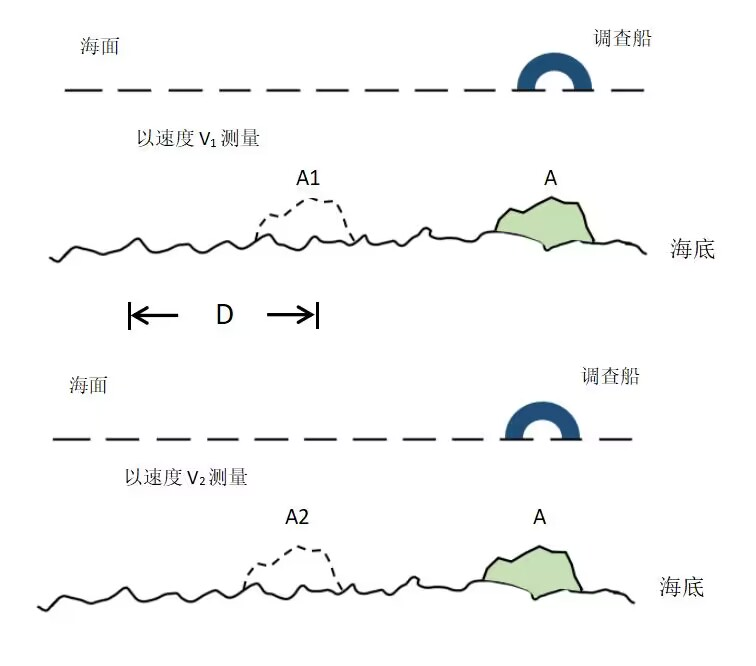
\includegraphics[width=.6\textwidth]{10}
    \caption{定位时间延迟分析}
    \label{fig:four}
\end{figure}
或使用下面公式进行误差消除或误差检验。该章节所述两个公式区别在于:前者可基于整个测量过程之后进行数据分析,而后者必须要测量时定点进行准确度的测算:[4]
\begin{equation}
\sigma=\pm\sqrt{\frac{\sum_{i=1}^{n}{(h_i-h)}^2}{n-1}}
\end{equation}
通过误差计算,可得到测量数据是否可靠准确。该误差与测点的水深测量值的平均值反应了该测深系统、算法与测量仪器的准确度。

若传感器由于某些原因(如噪声等)未能按时$t_0$接受到数据,只在$t_i$、$t_{i+1}$时刻接收到数据,则本文定义如下公式:基于线性插值的时间配准公式
\begin{equation}
y_0=\frac{t_0-t_i}{t_{i+1}-t_i}y_{i+1}+\frac{t_{i+1}-t_0}{t_{i+1}-t_i}y_i
\end{equation}
其中,$y_i$是该时刻采集到的声波传递时间的数据。
\subsubsection{横摇与纵倾的波浪分析与改进}
本节以横摇为例,介绍改进策略,纵倾的偏差分析原理近似。
横摇偏差($\phi$)一般是由装置安装偏差、波浪潮汐导致的船体运动等引起。由于波浪次数多、随机性强,因此后者引起的该偏差在统计学意义上为一常量。若多波束测量系统中存在横摇偏差,则在假定海平面表面平坦下,平均的垂直航迹就会发生微小偏移。一般情况下,正向测量与反向测量后,两者倾斜地形会形成对称的假象。

为了获取海浪潮汐引起的横摇偏差,测量获得的“测量的假地形”倾斜角度需要与横摇偏角统一正负关系。由于真实地形的坡度为定值,则两方向的地形剖面倾角的算术平均数即为横摇偏差,可用下面的公式简单表示单位为度:
\begin{equation}
\phi=\frac{\phi_1+\phi_2}{2}
\end{equation}
\subsubsection{潮位分析与改进}
对于潮位不同产生的海拔水位的误差,我们在测量时得到自然月或自然日中取多次测量,最后取平均值即可。此外,也可通过潮水规律进行分析和计算。
\subsection{模型推广}
本文较为完整的分析了在多波束测量海底地形的应用场景下,各种不同规划方法下测量方式的最优解。较为完整的分析了多种因素对最终测量结果的影响,如地形坡度、测量路线、测线间距等。且通过严格的数学推导证明了其可行性与必要性。不仅提供了实际测绘工作中较为可行的方法,也提供了误差分析、测量算法评价的方式,为测绘提供了较强的借鉴意义。

此外,在实际研究中,我们需要根据实际情况来进行合理抽象化与理想化,如声音在介质中的衍射等。



\begin{thebibliography}{9}%宽度9
    \bibitem[1]{a}
    中国地址调查局 地址调查技术标准 DD2012-01
    \newblock 北京\allowbreak[S].
    \newblock 中国地址调查局, 2012.
    \bibitem[2]{b}
	基于多波束声纳海底测量数据构建三维地形模型的方法
    \newblock 黑龙江\allowbreak[P].
    \newblock 哈尔滨工程大学,王宏健,2011.
	\bibitem[3]{c}
	基于相位法的多波束声呐海底地形测量质量实时评估方法
    \newblock 黑龙江\allowbreak[M].
    \newblock 哈尔滨工程大学,杜伟东, 周天, 王璐瑶, 徐超, 陈宝伟,2023.
	\bibitem[4]{c}
	多波束测深系统的精度评估方法研究
    \newblock 重庆\allowbreak[M].
    \newblock 《海洋技术》,吴英姿, 徐新盛, 乔力争,2003.

\end{thebibliography}

\newpage
%附录
\begin{appendices}
\section{支撑材料文件列表}
\begin{table}[!htbp]
    \caption{支撑材料列表}\label{tab:001} \centering
    \begin{tabular}{ccccc}
        \toprule[1.5pt]
        文件名 & 备注\\
        \midrule[1pt]
        result1.xlsx&问题一结果\\
	result2.xlsx&问题二结果\\
	第一问.py&问题一Python代码\\
	第二问.py&问题二Python代码\\
	第三问.py&问题三Python代码\\
	第四问.py&问题四Python代码第一部分\\
	第四问2.py&问题四Python代码第二部分\\
	第三问答案.csv&问题三答案\\
	第四问地形图模拟.py&问题四地形图Python代码\\
	附件.xlsx&该问题附件\\
        \bottomrule[1.5pt]
    \end{tabular}
\end{table}

\section{结果展示}
\begin{table}[H]
    \caption{第三问结果}\label{tab:001} \centering
\resizebox{0.3\textwidth}{0.5\textheight}{
    \begin{tabular}{ccccc}
        \hline
        $x_i$ & $W_i$  & -\\
        \hline
        3345.536203	&686.1015914&	1\\
2750.584887	&631.9927325	&2\\
2202.484662	&582.1448258	&3\\
1697.54611	&536.2223308	&4\\
1232.370345&	493.9161301	&5\\
803.8261365&	454.9414485&	6\\
409.0288301	&419.0359363&	7\\
45.3209328	&385.9579033&	8\\
-289.7457772	&355.4846917&	9\\
-598.4267297&	327.4111777&	10\\
-882.7997443	&301.5483905&	11\\
-1144.779017	&277.7222402&	12\\
-1386.128005	&255.7723461&	13\\
-1608.471298	&235.5509574&	14\\\
-1813.305551&	216.921958	&15\\
-2002.009563&	199.7599509&	16\\
-2175.853554	&183.9494136&	17\\
-2336.007717	&169.3839209&	18\\
-2483.550097	&155.9654284	&19\\
-2619.473843	&143.6036123&	20\\
-2744.693896&	132.2152616	&21\\
-2860.053149&	121.7237183&	22\\
-2966.328117&	112.0583606&	23\\
-3064.234169&	103.1541283&	24\\
-3154.430336	&94.95108452&	25\\
-3237.523757	&87.39401216&	26\\
-3314.073755&	80.43204242&	27\\
-3384.595611&	74.0183123&	28\\
-3449.564029&	68.10964915	&29\\
-3509.416328&	62.66628007&	30\\
-3564.555391	&57.65156419	&31\\
-3615.352376	&53.03174602&	32\\
-3662.149212	&48.77572825&	33\\
-3704.260901	&44.8548624	&34\\
        \hline
    \end{tabular}}
\end{table}
\section{核心代码}

\begin{tcode}
#第一问
import math

def calculate_coverage_width(D, theta, alpha):
    theta = math.radians(theta)
    alpha = math.radians(alpha)
    W1 = abs((D*math.tan(theta))/(1-math.tan(theta)*math.tan(alpha)))
    W2 = abs((D * math.tan(theta)) / (1 + math.tan(theta) * math.tan(alpha)))
    print(W1)
    print(W2)
    return W1+W2

def calculate_coverage_width2(D, theta, alpha):
    theta=math.radians(theta)
    alpha=math.radians(alpha)
    W2 = abs((D * math.tan(theta)) / (1 + math.tan(theta) * math.tan(alpha)))
    return W2
def calculate_overlap_rate(W0,W1, distance,right):
    eta = (W0+right-distance)/W1
    return eta

def calculate_depth(h,alpha):
    alpha=math.radians(alpha)
    a=70-h*math.tan(alpha)
    return a

def main():
    theta = 120/2
    alpha = 1.5
    distance=200#测线间距步长
    h=-800#距中心的距离我们要改这里
    W0 = 200#之前的右半个宽度,我们要改这里
    a = calculate_depth(h, alpha)
    W1 = calculate_coverage_width(a, theta, alpha)
    d = W0 + W1 - distance  # 重叠部分面积
    right=calculate_coverage_width2(a, theta, alpha)
    eta = calculate_overlap_rate(W0,W1, distance,right)

    print(f"覆盖宽度 W: {W1:.2f} 米")
    print(f"深度 height: {a:.2f} 米")
    print(f"重叠率 eta: {eta * 100:.2f}%")

if __name__ == "__main__":
    main()


#第二问
import math

beam_angle_deg = 60  
slope_deg = 1.5  
center_depth = 120 )
beta_deg = 315  
distance_to_center =2.1*1852  

# 将角度转换为弧度
beam_angle_rad = math.radians(beam_angle_deg)
slope_rad = math.radians(slope_deg)
beta_rad = math.radians(beta_deg)

deltaz=distance_to_center*math.cos(beta_rad)*math.tan(slope_rad)
depth=center_depth+deltaz
print(depth)
tanGama=math.sin(beta_rad)*math.tan(slope_rad)
print(tanGama)

# 计算波束覆盖宽度的数学模型
def calculate_beam_width(beam_angle_rad, slope_rad, beta_rad, depth):
    # 计算水深对应的波束覆盖宽度
    W1 = abs(
        (depth * math.tan(beam_angle_rad)) / (1 - math.tan(beam_angle_rad) *tanGama))
    W2 = abs(
        (depth * math.tan(beam_angle_rad)) / (1 + math.tan(beam_angle_rad) *tanGama))
    beam_width = W1+W2
    print(W1)
    print(W2)
    return beam_width

a=calculate_beam_width(beam_angle_rad, slope_rad,beta_rad, depth)
coverage_width = calculate_beam_width(beam_angle_rad, slope_rad, beta_rad,depth)
overlap_percentage = 15  
d = coverage_width * (100 / overlap_percentage - 1)

print(f"多波束测深的覆盖宽度:{a:.2f} 米")

#第三问代码
def generate_x_sequence(k, b, k1, b1, k2, b2):
    x_sequence = []
    x_0 = (2 * 1852  - b1) / (1 + k1)
    x_sequence.append(x_0)

    while True:
        x_i = x_sequence[-1]
        next_x= (k2-1)*x_i/(0.1*k-k1-1)+(b1+b2-0.1*b)/(0.1*k-k1-1)
        if next_x < x_i:
            x_sequence.append(next_x)
            if next_x <= -2 * 1852 and next_x - k2 * next_x - b2 <= -2 * 1852:
                break
        else:
            break

    return x_sequence

k = 0.0909467
b = 381.836114
k1 = 0.047493  
b1 = 199.5742463  
k2 = 0.043373227  
b2 = 182.836114

x_sequence = generate_x_sequence(k, b, k1, b1, k2, b2)

total_W = 0

for i, x in enumerate(x_sequence):
    W_i = k * x + b
    print(f'x_{i} = {x}, W_{i} = {W_i}')
    if i <= 33:
        total_W += W_i

print(f'Total sum of W_0 to W_32: {total_W}')

#第四问代码
from matplotlib import pyplot as plt
import numpy as np
import pandas as pd
from mpl_toolkits.mplot3d import Axes3D
import warnings
warnings.filterwarnings("ignore", category=UserWarning)
from scipy import interpolate

###########导入数据,初始化,网格化#########################
data = pd.read_excel(r"C:/Users/MMinuzero/Desktop/B题/附件.xlsx")

x=data.iloc[0:1, 2:203].values
y=data.iloc[1:253, 1:2].values
X = np.array(x)
Y = np.array(y)
X, Y = np.meshgrid(X, Y)
print("网格化后的X=",X)
print("X维度信息",X.shape)
print("网格化后的Y=",Y)
print("Y维度信息", Y.shape)
z=data.iloc[1:253, 2:203].values
Z = np.array(z)
print("网格化后的Z=",Z)
print("Z轴数据维度",Z.shape)

##########依据等高线选代表梯度的点#########################
# 找到最大的z值及其对应的坐标
max_z = np.max(Z)
max_indices = np.argwhere(Z == max_z)
x_0, y_0 = X[max_indices[0][0], max_indices[0][1]], Y[max_indices[0][0], max_indices[0][1]]

# 打印z值最大的点的坐标,并标注为A点
print(f"A点坐标:({x_0}, {y_0}, {max_z})")

# 设置步长d和弹性范围c
d = 10
c = 0.3

# 初始化结果列表
selected_points = []

# 开始搜索最近的点
z_i = max_z
while True:
    z_i -= d
    z_min = z_i - c
    z_max = z_i + c
    
    # 找到z范围内的点
    within_range_indices = np.argwhere((Z >= z_min) & (Z <= z_max))
    
    if len(within_range_indices) == 0:
        break  # 如果没有点在范围内,退出循环
    
    # 计算距离最近的点
    distances = np.sqrt((X[within_range_indices[:, 0], within_range_indices[:, 1]] - x_0)**2 +
                        (Y[within_range_indices[:, 0], within_range_indices[:, 1]] - y_0)**2 +
                        (Z[within_range_indices[:, 0], within_range_indices[:, 1]] - z_i)**2)
    min_distance_index = np.argmin(distances)
    
    # 获取最近点的坐标
    x_i, y_i, z_i = X[within_range_indices[min_distance_index][0],within_range_indices[min_distance_index][1]],Y[within_range_indices[min_distance_index][0],within_range_indices[min_distance_index][1]], Z[within_range_indices[min_distance_index][0], within_range_indices[min_distance_index][1]]
    
    # 添加到结果列表
    selected_points.append((x_i, y_i, z_i))

# 重新编号所选点
for i, (x_i, y_i, z_i) in enumerate(selected_points):
    print(f"A_{i+1}坐标:({x_i}, {y_i}, {z_i})")

#########################可视化选点结果############################

# 提取selected_points中的z值并排序
z_values = sorted(list(set([point[2] for point in selected_points])))

# 在等高线图上绘制等高线,使用排序后的z值
plt.contourf(X, Y, Z, levels=z_values + [z_values[-1] + 1], cmap='viridis')
plt.colorbar()

# 绘制选定的点及其投影坐标
for i, (x_i, y_i, z_i) in enumerate(selected_points):
    # 绘制选定点的标记
    plt.scatter(x_i, y_i, c='red', label=f'A_{i+1}', s=50, zorder=3)

# 设置y轴数据范围为(0,5)
plt.ylim(0, 5)

# 设置图形属性
plt.xlabel('X')
plt.ylabel('Y')
plt.title('contour map')
plt.legend()
plt.grid(True)
plt.show()

##################做拟合,找梯度方向########################
# 提取A点的x和y坐标
x_coords = [point[0] for point in selected_points]
y_coords = [point[1] for point in selected_points]

# 进行线性回归
coefficients = np.polyfit(x_coords, y_coords, 1)
slope, intercept = coefficients

# 创建拟合直线的x值范围
x_fit = np.linspace(min(x_coords), max(x_coords), 100)
y_fit = slope * x_fit + intercept

# 绘制等高线图
plt.contourf(X, Y, Z, levels=z_values + [z_values[-1] + 1], cmap='viridis')
plt.colorbar()

# 绘制选定的点及其投影坐标
for i, (x_i, y_i, z_i) in enumerate(selected_points):
    # 绘制选定点的标记
    plt.scatter(x_i, y_i, c='red', label=f'A_{i+1}', s=50, zorder=3)
    
# 绘制线性回归的拟合直线
plt.plot(x_fit, y_fit, 'b-', label=f'Linear Fit (y = {slope:.2f}x + {intercept:.2f})', lw=2)

# 设置y轴数据范围为(0,5)
plt.ylim(0, 5)
#记录拟合直线数据
y = -0.15 * x + 0.69

# 设置图形属性
plt.xlabel('X轴')
plt.ylabel('Y轴')
plt.title('Linear fitting')
plt.legend()
plt.grid(True)
plt.show()

##########################找B_j#############################
# 初始化结果列表
selected_B_j_points = []

# 遍历 X、Y、Z 数据
for i in range(X.shape[0]):
    for j in range(X.shape[1]):
        x_i = X[i, j]
        y_i = Y[i, j]
        z_i = Z[i, j]
        
        # 计算每个点的 y_j 值
        calculated_y_j = -0.15 * x_i + 0.69
        
        # 检查是否满足条件
        if abs(calculated_y_j - y_i) < 1e-6:  # 使用小误差来比较浮点数
            selected_B_j_points.append((x_i, y_i, z_i))

# 按照 x_j 从小到大的顺序对点进行排序
sorted_B_j_points = sorted(selected_B_j_points, key=lambda point: point[0])

# 打印排序后的 B_j 点
for i, (x_j, y_j, z_j) in enumerate(sorted_B_j_points):
    print(f"B_{i+1}坐标:({x_j}, {y_j}, {z_j})")

##############定义第j条测线在xoy平面投影的表达式###############
#y = (1/0.15) * (x - x_j) + y_j  ####斜率6.66,网格化B_j两侧做3*2网格

##############定义梯度拟合线上点B_j处的坡度###############
# 初始化结果列表
selected_B_j_points = []

# 遍历 X、Y、Z 数据
for i in range(X.shape[0]):
    for j in range(X.shape[1]):
        x_i = X[i, j]
        y_i = Y[i, j]
        z_i = Z[i, j]
        
        # 计算每个点的 y_j 值
        calculated_y_j = -0.15 * x_i + 0.69
        
        # 检查是否满足条件
        if abs(calculated_y_j - y_i) < 1e-6:  # 使用小误差来比较浮点数
            selected_B_j_points.append((x_i, y_i, z_i))

# 按照 x_j 从小到大的顺序对点进行排序
sorted_B_j_points = sorted(selected_B_j_points, key=lambda point: point[0])

# 打印排序后的 B_j 点
for i, (x_j, y_j, z_j) in enumerate(sorted_B_j_points):
    print(f"B_{i+1}坐标:({x_j}, {y_j}, {z_j})")
########################插值############################
# 将 B_j 点的坐标拆分成 x、y、z 列表
x_j_values = [point[0] for point in sorted_B_j_points]
y_j_values = [point[1] for point in sorted_B_j_points]
z_j_values = [point for point in sorted_B_j_points]

# 创建一个列表,用于存储插值后的点
interpolated_points = []

# 在相邻的 B_j 点之间进行插值
for i in range(len(x_j_values) - 1):
    num_interpolated_points = 20  # 插入的点数
    x_interp = np.linspace(x_j_values[i], x_j_values[i + 1], num_interpolated_points)
    y_interp = np.linspace(y_j_values[i], y_j_values[i + 1], num_interpolated_points)
    z_interp = np.linspace(z_j_values[i], z_j_values[i + 1], num_interpolated_points)
    
    # 将插值结果添加到列表中
    interpolated_points.extend(list(zip(x_interp, y_interp, z_interp)))

# 合并原始 B_j 点和插值后的点
all_points = sorted_B_j_points + interpolated_points

# 使用 sorted 函数按照 x 值从大到小排序
sorted_all_points = sorted(all_points, key=lambda point: point[0], reverse=True)

# 为排列后的点标记为C_m
C_m_points = [(f'C_{i}', x_i, y_i, z_i) for i, (x_i, y_i, z_i) in enumerate(sorted_all_points, start=1)]

# 创建一个列表,用于存储 C_m 的信息
C_m = []

# 输出标记后的点
for label, x_i, y_i, z_i in C_m_points:
    # 将坐标信息添加到 C_m 列表中
    C_m.append({'x_m': x_i, 'y_m': y_i, 'z_m': z_i})

# 输出标记后的点
for label, x_i, y_i, z_i in C_m_points:
    print(f"{label}坐标:({x_i}, {y_i}, {z_i})")
################定义坡度##################
# 计算每个 C_m 点的坡度
slope_values = []
for i in range(5, len(C_m_points) - 5):
    x_m = C_m_points[i][1]
    y_m = C_m_points[i][2]
    z_m_minus_5 = C_m_points[i - 5][3]
    z_m_plus_5 = C_m_points[i + 5][3]
    distance_squared = (C_m_points[i + 5][1] - C_m_points[i - 5][1])**2 + (C_m_points[i + 5][2] - C_m_points[i - 5][2])**2
    tana_m = (z_m_minus_5 - z_m_plus_5) / (1852 * np.sqrt(distance_squared))
    slope_values.append(tana_m)

# 打印每个 C_m 点的坡度值
for i, slope in enumerate(slope_values, start=5):
    print(f"C_{i}点的坡度 (tana_m):{slope:.4f}")

################定义C_m处的覆盖宽度########################
# 存储覆盖宽度1(W1_m)和覆盖宽度2(W2_m)的值
W1_values = []
W2_values = []
# 存储 C_m 点的坐标和宽度信息
C_m = []

# 计算每个 C_m 点的 W1_m 和 W2_m
for i in range(5, len(C_m_points) - 5):
    z_m = C_m_points[i][3]
    tana_m = slope_values[i - 5]
    
    # 计算覆盖宽度1(W1_m)
    W1_m = (z_m * np.sqrt(3)) / (1 - 3 * tana_m)/1852
    
    # 计算覆盖宽度2(W2_m)
    W2_m = (z_m * np.sqrt(3)) / (1 + 3 * tana_m)/1852
    
    # 将坐标和宽度信息添加到 C_m 列表中
    C_m.append({'x_m': C_m_points[i][1], 'y_m': C_m_points[i][2], 'z_m': z_m, 'W1_m': W1_m, 'W2_m': W2_m})

# 打印每个 C_m 点的坐标、W1_m 和 W2_m 值
for i, point in enumerate(C_m, start=5):
    print(f"C_{i}坐标:(x_m={point['x_m']}, y_m={point['y_m']}, z_m={point['z_m']}), W1_m={point['W1_m']:.4f}, W2_m={point['W2_m']:.4f}")
    # 存储到相应的列表中
    W1_values.append(W1_m)
    W2_values.append(W2_m)

# 打印每个 C_m 点的 W1_m 和 W2_m 值
for i, (W1, W2) in enumerate(zip(W1_values, W2_values), start=5):
    print(f"C_{i}点的覆盖宽度1 (W1_m):{W1:.4f}")
    print(f"C_{i}点的覆盖宽度2 (W2_m):{W2:.4f}")

###############选择测线##########################
# 初始化选定的C_m点
selected_C_m = None
max_distance = 0  # 用于跟踪最远距离

# 假设D0点的坐标为 (x_1, y_1)
x_1 = C_m_points[0][1]
y_1 = C_m_points[0][2]

# 计算D0点的覆盖宽度1(W1_1)和覆盖宽度2(W2_1)
W1_1 = W1_values[0] if len(W1_values) > 0 else 0
W2_1 = W2_values[0] if len(W2_values) > 0 else 0

# 遍历C_m点,查找满足条件的点
for i in range(len(C_m_points)):
    x_m1 = C_m_points[i][1]
    y_m1 = C_m_points[i][2]
    
    # 确保索引在有效范围内
    if i < len(W1_values) and i < len(W2_values):
        W1_m1 = W1_values[i]
        W2_m1 = W2_values[i]
        
        # 计算条件的值
        condition_value = (W2_1 + W1_m - np.sqrt((x_1 - x_m1)**2 + (y_1 - y_m1)**2)) / (W1_m + W2_m)
        
        # 检查是否满足条件
        if 0.13 <= condition_value <= 0.17:
            # 计算距离D0点的距离
            distance_to_D0 = np.sqrt((x_1 - x_m1)**2 + (y_1 - y_m1)**2)
            
            # 如果距离更远,更新选定的C_m点和最远距离
            if distance_to_D0 > max_distance:
                selected_C_m = C_m_points[i]
                max_distance = distance_to_D0

if selected_C_m is not None:
    print(f"选择的C_m点坐标:({selected_C_m[1]}, {selected_C_m[2]}, {selected_C_m[3]})")
else:
    print("未找到满足条件的C_m点。")  


\end{tcode}
\begin{figure}[H]
    \centering
    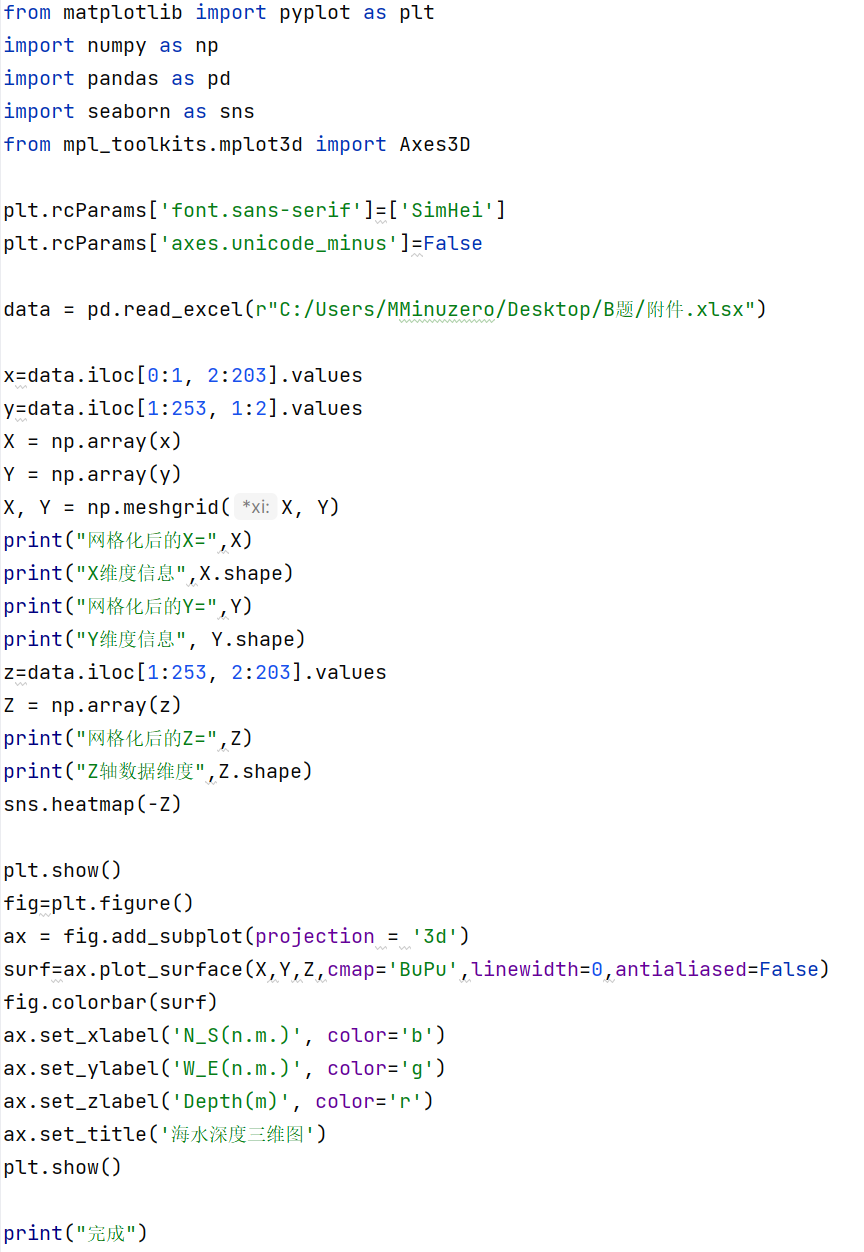
\includegraphics[width=.9\textwidth]{16}
    \caption{画图代码 第四问立体图}
    \label{fig:four}
\end{figure}


\end{appendices}

\end{document} 